\chapter{Analysis}

\section{Introduction}

\subsection{Client Identification}

	\begin{flushleft}

		My client is 30 year old plasterer Dan Austin who runs his own plastering business known as DnA Plastering. Dan mainly uses his Toshiba laptop (Dual Core Intel with 6 GB Ram and running Windows 8 64 bit) to do basic tasks such as social networking and receiving/sending emails. \par

The current system is a paper based method where he records the prices and measurements of the plastering/screening/rendering jobs he undertakes. Dan works in an around the Suffolk/Essex area but occasionally takes on larger jobs further afield in places such as London or Epping. All the recording and calculations are done by Dan himself and does not require additional assistance in completing these tasks but is looking for a digital solution to the organisation problems faced with the current manual paper method. \par

Dan is looking to introduce a computer based system to replace the current one in order to make keeping track of jobs and pricing up new jobs easier and more efficient. Alongside this he would like to be able to keep information on all of his customers so he can simply search for clients' details and contact information all in one location. He will also be able to look up the jobs that he has done for them to make sending invoices easier and manageable.

		
	\end{flushleft}

\subsection{Define the current system}

	\begin{flushleft}

	The current system in place is a paper/notebook based system where details of clients are stored along with prices of jobs and cost of materials needed etc. The details of the clients include their address, phone number, email, first name and surname. The infromation about the job usually includes the measurements of what needs to be plastered along with how long it will take to complete and if he is taking any labourers to too. Calculations are often also made to work out how much to charge depending on the price he is charging per square meter. This rate often changes depending on the current economy. \par

Once all the calculations are made, he works out how much the materials are going to cost and also how long it will take him to complete the job. Once all these calculations and prices have been evaluated he notifies the client of the price; when the price is confirmed the job is undertaken.	 \par

Finally, Dan writes out an invoice using a standard invoice book purchased from a stationary store to inform the client of the costs and charges of the job. The current folder containing the invoices for his clients is not organised and offers another problem whereby finding information for jobs is difficult due to the inability to search quickly for any given customer.
		
	




	\end{flushleft}

\subsection{Describe the problems}


	\begin{flushleft}
	
	Problems are plentiful in the current system. One of the main problems is keeping valuable client data from being lost or damaged as there is only one hard copy made in a notebook. Another problem with the notebook is not being able to easily search through the details of all the clients to find specific phone numbers or contact details. Using a computer based system would allow Dan to search through his clients efficiently and allow him to make backups of the valuable client and job data. \par 
		



	
	\end{flushleft}

		





\subsection{Section appendix}


\begin{flushleft}
	\textbf{Interview with client}
\end{flushleft}


\begin{enumerate}
	\item \textbf{What system are you currently using?}
		\\ \\ I've got a Toshiba laptop with Windows 8, 6GB RAM and a dual core processor
	\item \textbf{Are there any issues with the system currently being employed?}
		\\ \\Just organisational issues when it comes to finding clients information etc. Would be good to have a database which I could search for info with.
	\item \textbf{What data do you record at the moment?}
		\\ \\ The clients name, address, phone number, job information like measurements of the rooms etc.
	\item \textbf{How often do you record data in the current system and how much data is stored each time?}
		\\ \\ A few times a week and not much, a few lines in the workbook I use.
	\item \textbf{What happens to older client information?}
		\\ \\ Normally gets lost as and when I replace any of my books I write the details down in.
	\item \textbf{Are there any storage issues when it comes to storing data manually?}
		\\ \\ No, nothing really as I only need room for a book or two.
	\item \textbf{Are changes often made to existing records of client data or job info?}
		\\ \\ Occasionally when a client gives me a new contact number but nothing major.
	\item \textbf{What is the typical routine when it comes to gaining a new client or job?}
		\\ \\ Normally I get a call from a colleague who gives me the details about a job which I can take on or not depending on the time I have available. Sometimes clients will find my number through my website dnaplastering.co.uk or through word of mouth and will ask me to give them a quote on a job. Then I will go to the job and work out any costs involved and the time it would take to complete. Then I can arrange a time to do the job and after the job is completed I will usually write out an invoice for the client telling them about the cost for materials,labouring and profit etc.
	\item \textbf{What does the client recieve in terms of invoices?}
		\\ \\ I write out an invoice and give it to them in person after the job is completed.
	\item \textbf{What format should the outputs be in within the new system?}
		\\ \\ It would be good to be able to print the clients invoices out with minimal effort involved and possibly email the clients the invoice.
	\item \textbf{Will you need to print reports and invoices or will it be sent entirely digitally to the client via email?}
		\\ \\ I definitely need to print out some of the invoices as most of my work is done face to face so it is easier to give it to them in person. It might be useful to email it to them as well.
	\item \textbf{Is there a security issue in regards to the data you store in the current system?}
		\\ \\ Not much of an issues as it is just client information  but added security would be a bonus.
	\item \textbf{Are there any foreseeable constraints required in the proposed system?}
		\\ \\ None that I am aware of.
	\item \textbf{Do you have a picture in mind of what the new system could look like?}
		\\ \\ Not really bothered about the look of it too much anything that works as expected would be brilliant.
\end{enumerate}

\begin{flushleft}
	\textbf{Signed:}
\begin{figure}[H]
    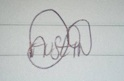
\includegraphics{./Analysis/images/signature.jpg}
\end{figure}

\end{flushleft}



\section{Investigation}

\subsection{The current system}
% Interview - Insert the transcript of the interview here.





\subsubsection{Data sources and destinations}


\begin{flushleft}
% Overview of the data sources and destinations
	There are four main data sources within the current system - The plasterer, the client, the builders merchant and visting the clients job. A client contacts Dan through a phone call placed to Dan's mobile. Sometimes a client may leave Dan a voicemail message if he is too busy to answer the call at that given moment. If this is the case then Dan will get back to the client as soon as possible. Most of the data in the current system will come from the client or the clients job - this data will be the job measurements and the clients contact information. The main data destinations are the forms given to the client i.e the quote and the invoice document.

\end{flushleft}

\begin{center}
	
    \begin{tabular}{|p{3cm}|p{3cm}|p{3cm}|p{3cm}|}
		\hline
		\textbf{Source} & \textbf{Data} & \textbf{Example Data} & 			 \textbf{Destination} \\

 \hline

        Client  &

			{Client Contact information Firstname - Lastname -  phoneNumber - AddrLine1 - 
AddrLine2 - AddrLine3 - AddrLine4 - PostCode - Email - JobType} & 

John - Smith - 07809726812 - 15 -  Crowley Road - Haverhill - Suffolk - CB90DJ - john@gmail.com - Plastering Bedroom &

Appointment and Client Book.
			
        \\
\hline

Plasterer &

Appointment Time and Place &

16:00 at 15 Crowley Road, Haverhill &

Client Calendar or Diary 

\\
\hline
Visiting Job Site &

Measurements of Job Size and Materials that need to be purchased &

4m x 5m x 3m = $60m^2$ 10 Bags of Plaster &

Work Notebook 

\\
\hline
Plasterers Calculations &

Quote for the work that needs doing and agree a date it can be done. &

\pounds 600, 1 Day, 15th October & 

Quote written out on paper or agree in person.

\\
\hline

Plasterers calculations for the materials needed for the job &

Quantity of materials needed for the job &

25 bags of plaster and 12m of angle beading &

Builders Merchant

\\
\hline
Builders Merchant &

A price for the materials needed &

\pounds 350 for the bags of plaster and angle beading &

Plasterer


\\
\hline

Plasterer &

Total cost of the job broken down - cost of parts,labouring and vat. Date of Job &

\pounds 600 - \pounds 350 materials - \pounds 50 VAT - 14/08/14 &

Client.

\\
        \hline
    \end{tabular}
\end{center}

\pagebreak
\subsubsection{Algorithms}
%Algorithms - Agreeing a price for the job - Calculating Job Price - Has the job been paid for yet.

There are three main algorithms utilised in the current system. The first is an algorithm to agree the price of the job with the client.

\begin{algorithm}[H]
\label{fig:algorithm_example_1}
	\caption{Agreeing a price Algorithm}
\begin{algorithmic}[1]

	\SET{$agreed$}{$false$}
	
	\While{agreed = False}
		\If{"Client does not agree with quoted price"} 
					\\ Discuss price and change quote if new price is agreed upon.\;
		\Else 
			\SET{$agreed$}{$true$}
			  \\ Arrange a date for the work to be started on.\;
		\EndIf
	\EndWhile

\end{algorithmic}
\end{algorithm}


The second algorithm currently being used in the system is an algorithm used to see whether the work is completed.


\begin{algorithm}[H]
	\label{fig:algorithm_work_complete}
		\caption{Checking whether work is complete or not.}
	\begin{algorithmic}[1]
		\SET{$Complete$}{$False$}
		\While{Complete = False}
			\If{"Issue/problem not fixed."}
			 \\ Check the current problem and fix issue.
			\Else
				\SET{$Complete$}{$True$}
			\EndIf
		\EndWhile
		\\Create and send invoice
	\end{algorithmic}
\end{algorithm}

The third algorithm being used in the system is an algorithm used to see whether the work has been paid for completely.


\begin{algorithm}[H]
	\label{fig:algorithm_paid}
		\caption{Checking whether work has been paid for yet.}
	\begin{algorithmic}[1]
		\SET{$Paid$}{$False$}
		\While{Paid = False}
			\If{"Money has not been given."}
			 \\ Send invoice and contact client
			\Else
				\SET{$Paid$}{$True$}
			\EndIf
		\EndWhile
		\\Update job to paid for in book.
	\end{algorithmic}
\end{algorithm}




\subsubsection{Data flow diagrams}

\textbf{Key}
\begin{figure}[H]
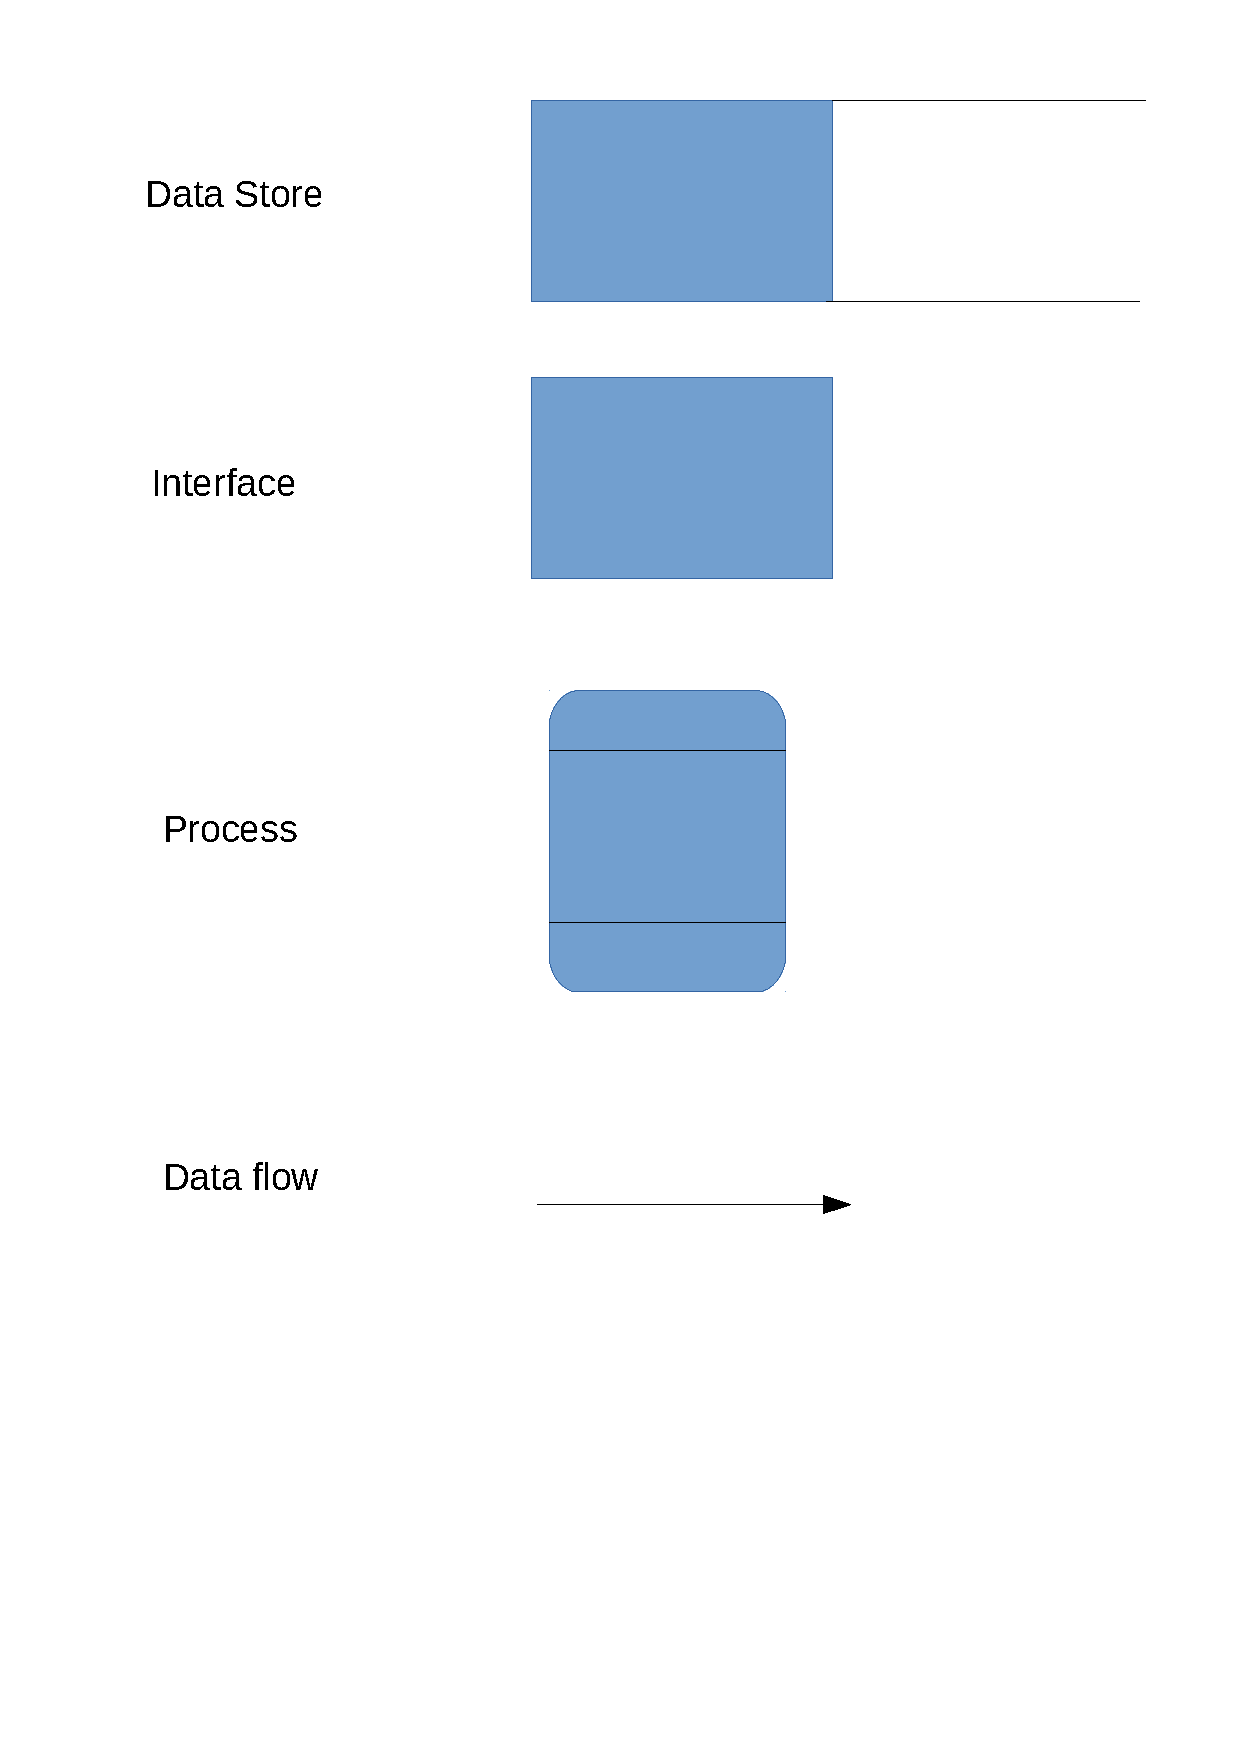
\includegraphics[width=\textwidth]{./Analysis/images/key.pdf}
    \caption{This is the Key to be used for the following data flow diagrams.} \label{fig:data_flow_diagram_key}
\end{figure}

\begin{figure}[H]
    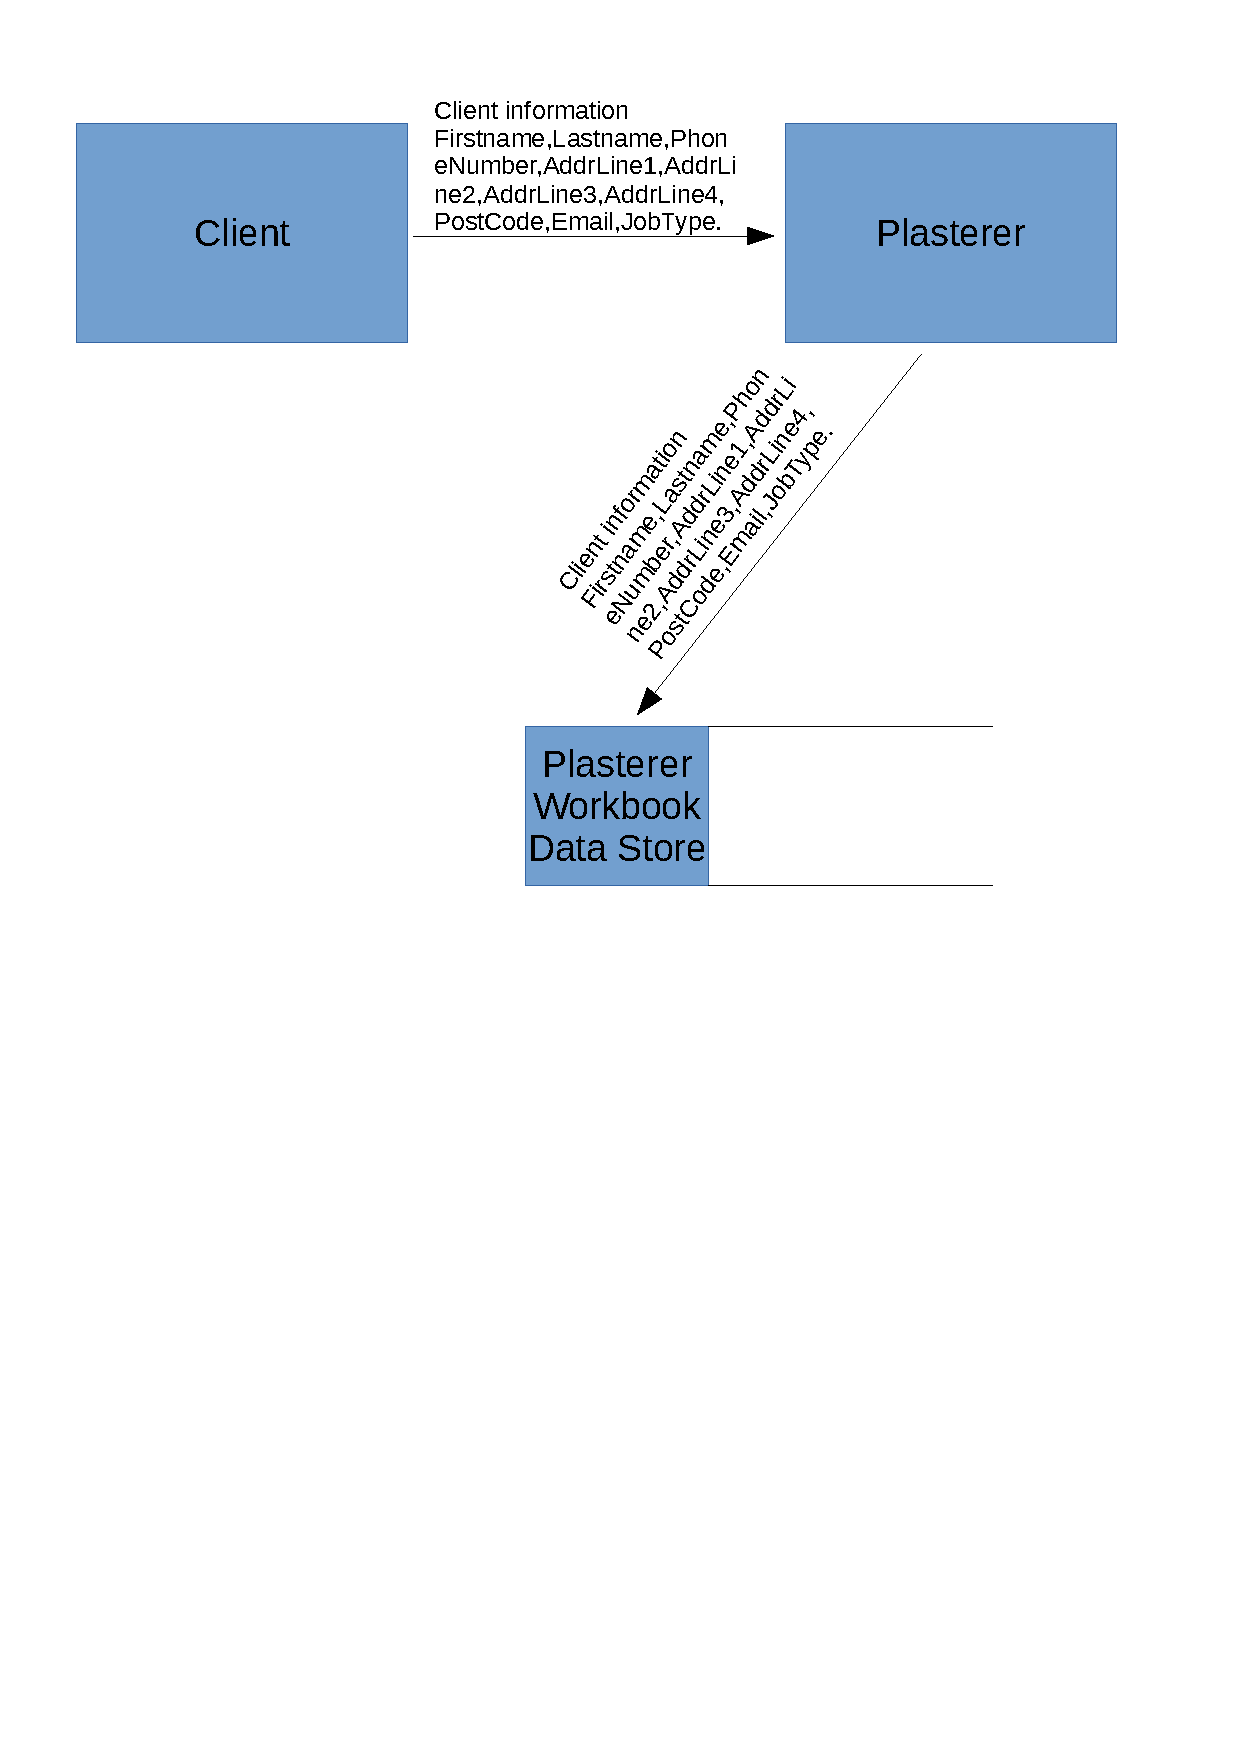
\includegraphics[width=\textwidth]{./Analysis/images/ClientInformation.pdf}
    \caption{This diagram shows the flow of data when gaining a new clients information.} \label{fig:client_information_data_flow_diagram}
\end{figure}

\begin{figure}[H]
    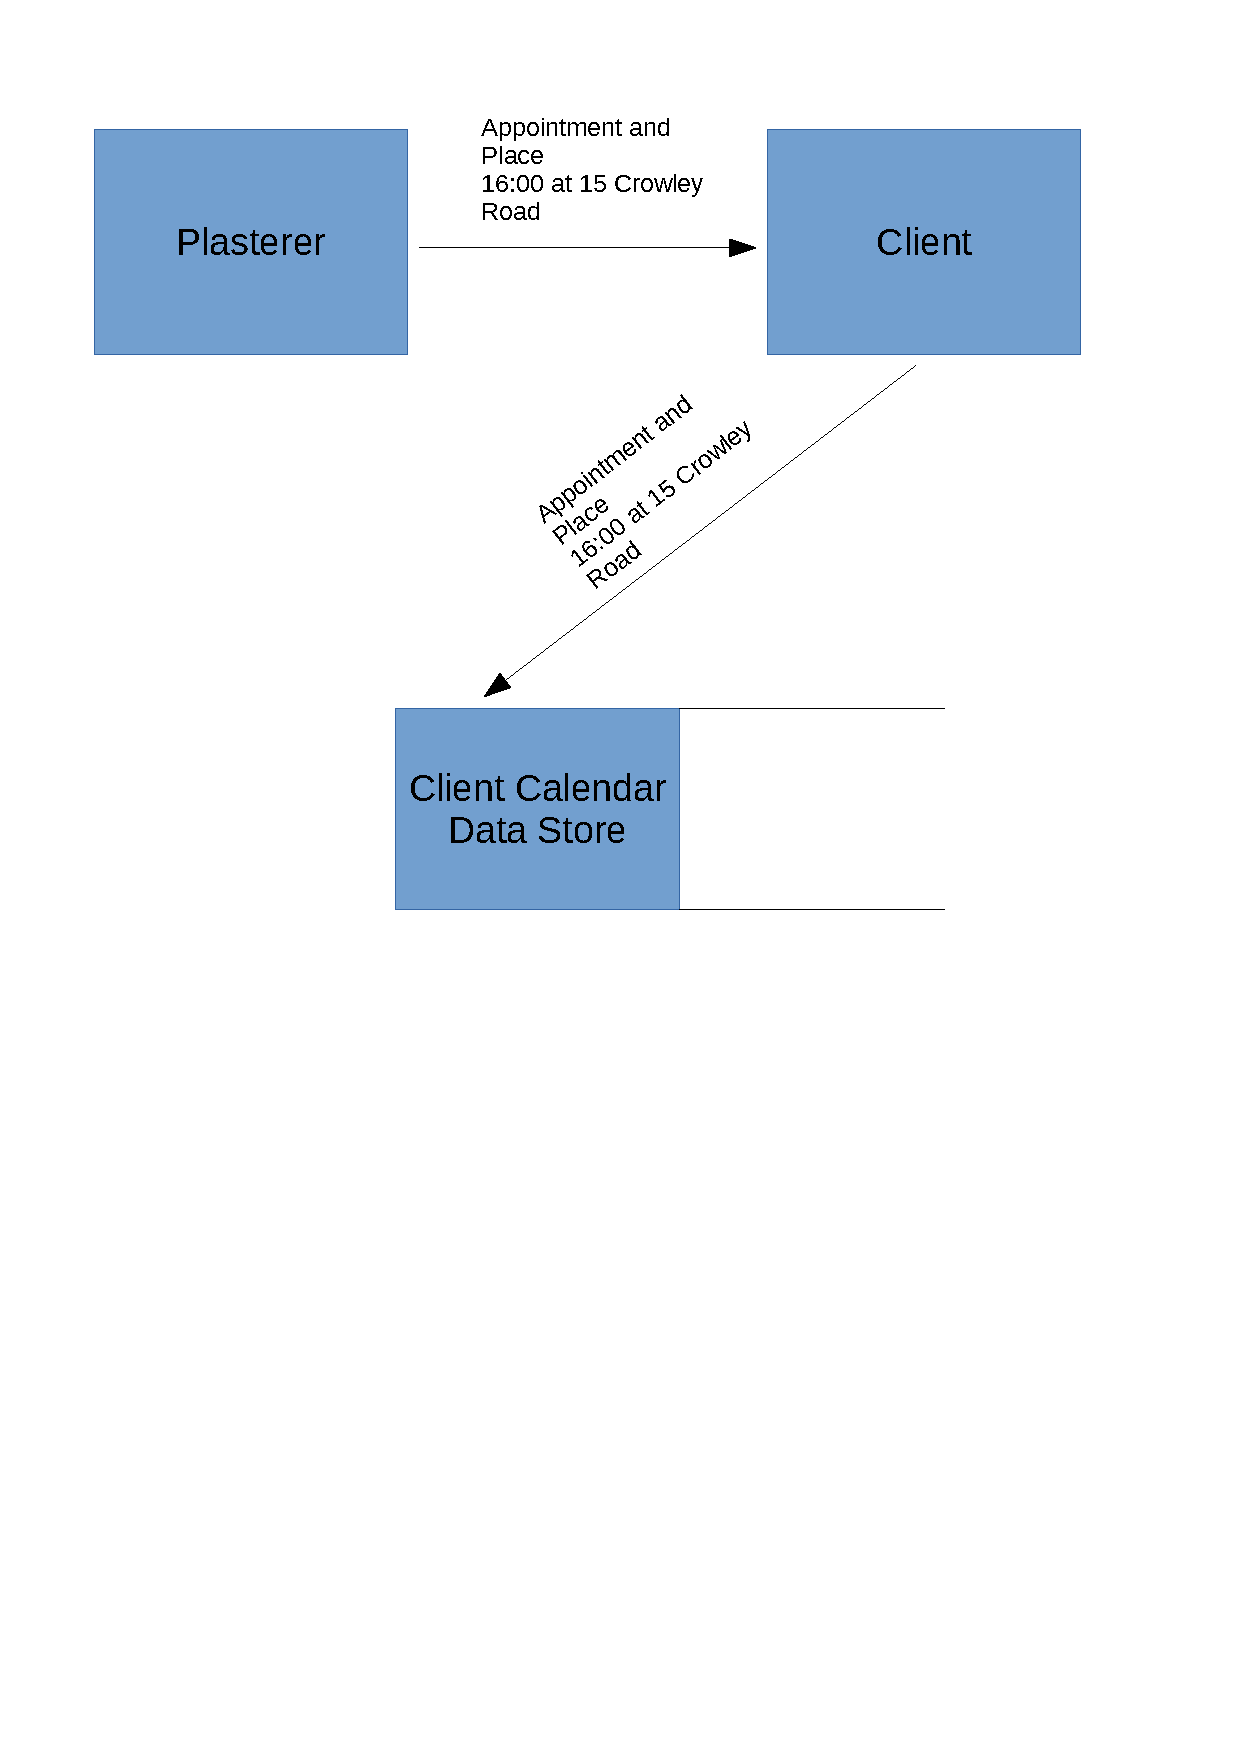
\includegraphics[width=\textwidth]{./Analysis/images/AppointmentDFD.pdf}
    \caption{The signifies the flow of data when making an appoint for a job.} \label{fig:appointment_data_flow_diagram}
\end{figure}

\begin{figure}[H]
    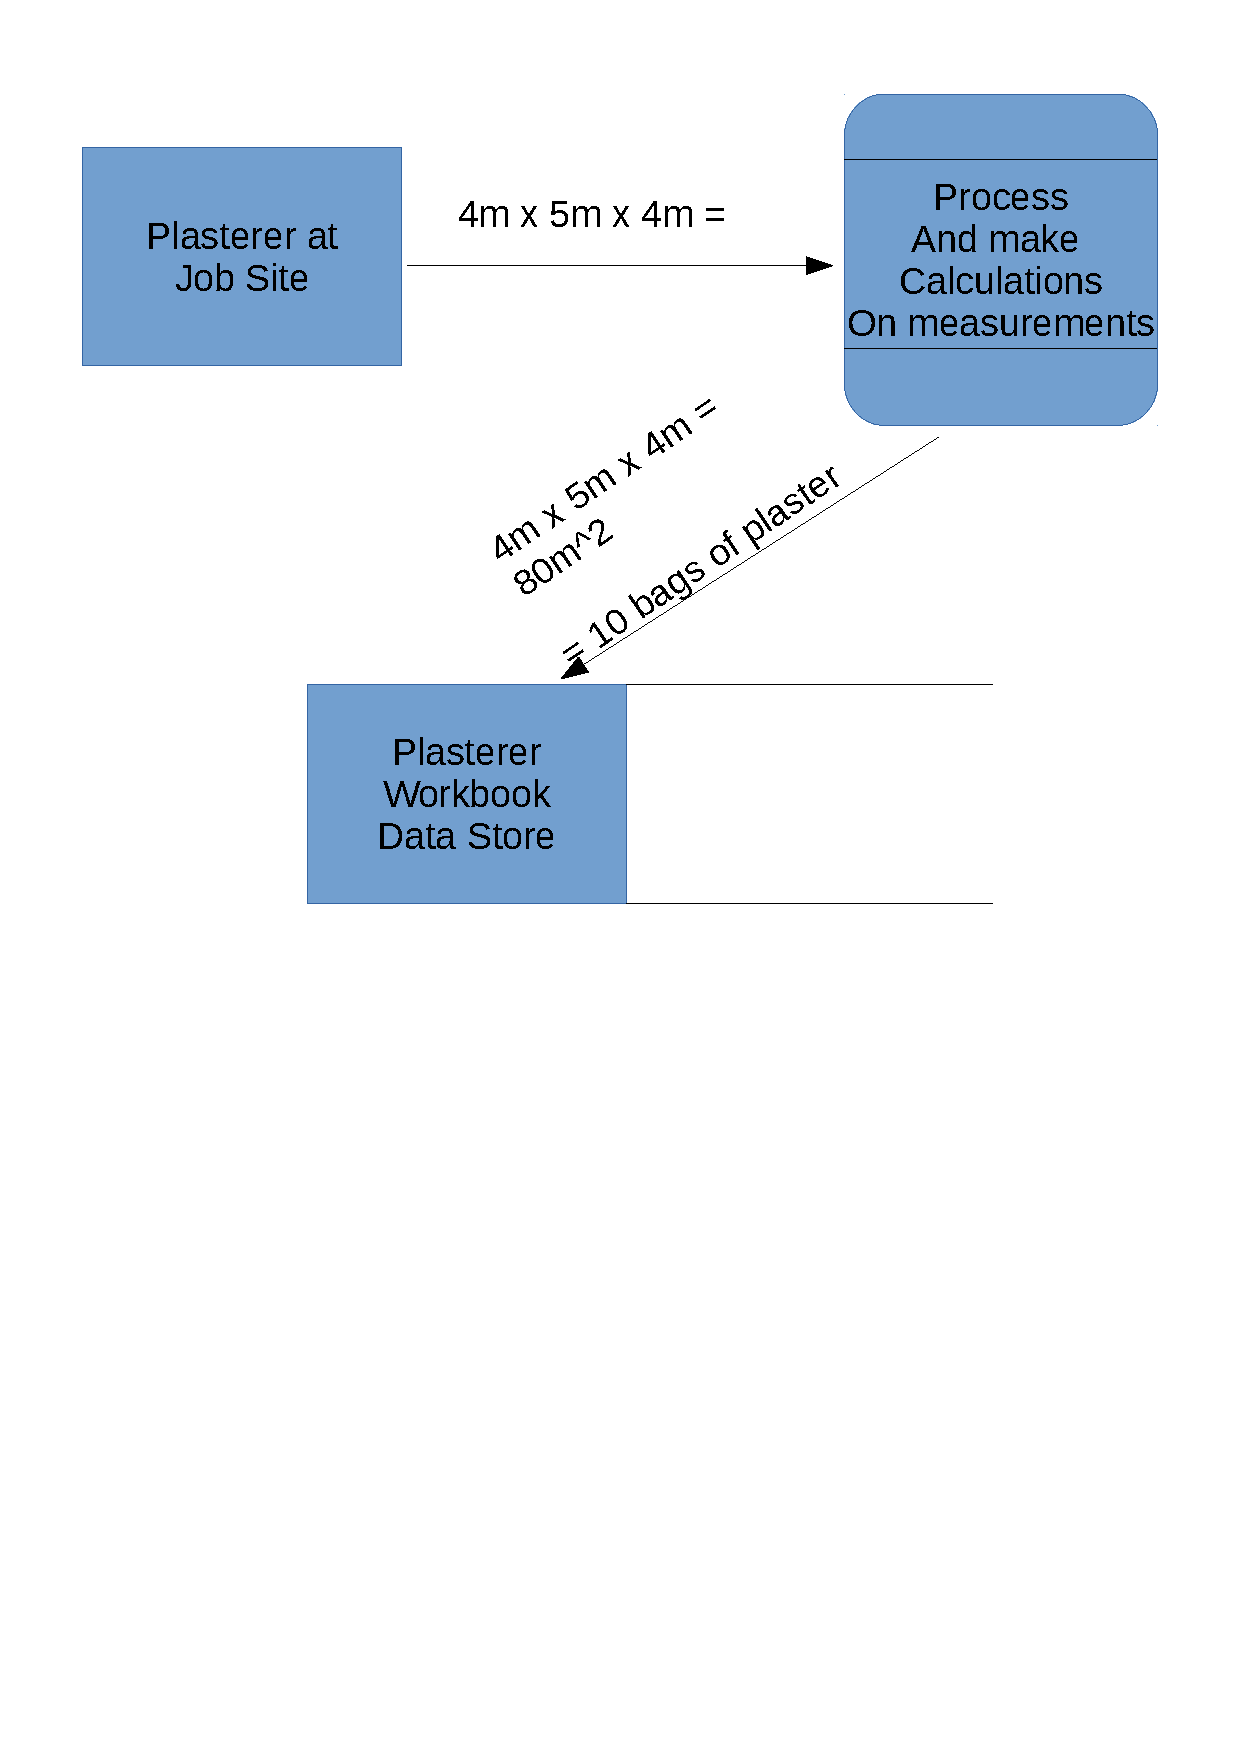
\includegraphics[width=\textwidth]{./Analysis/images/GettingMeasurements.pdf}
    \caption{This diagram shows the flow of data when collecting the measurements for a job.} \label{fig:getting_measurements_data_flow_diagram}
\end{figure}


\begin{figure}[H]
    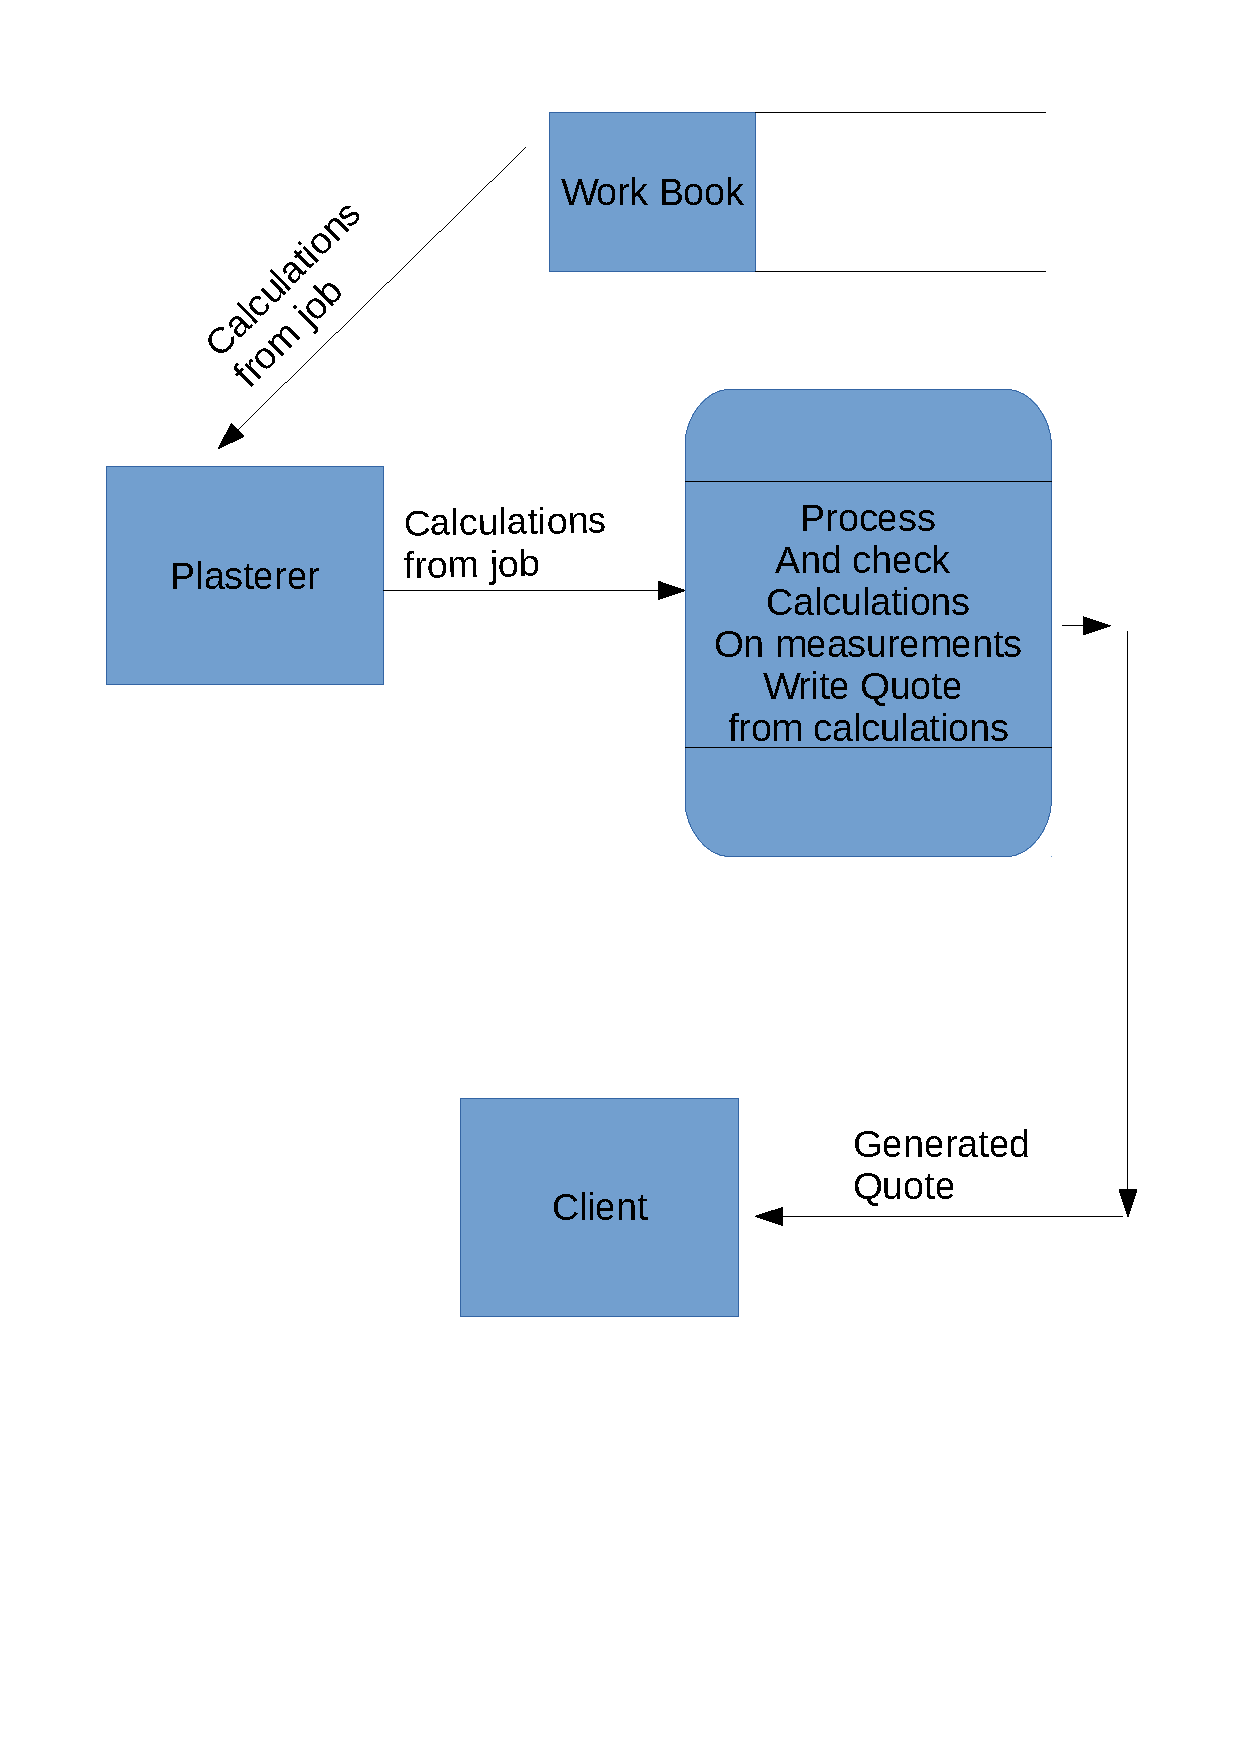
\includegraphics[width=\textwidth]{./Analysis/images/GeneratingQuote.pdf}
    \caption{The flow of data when generating a quote for the client.} \label{fig:generating_quote_data_flow_diagram}
\end{figure}

\begin{figure}[H]
    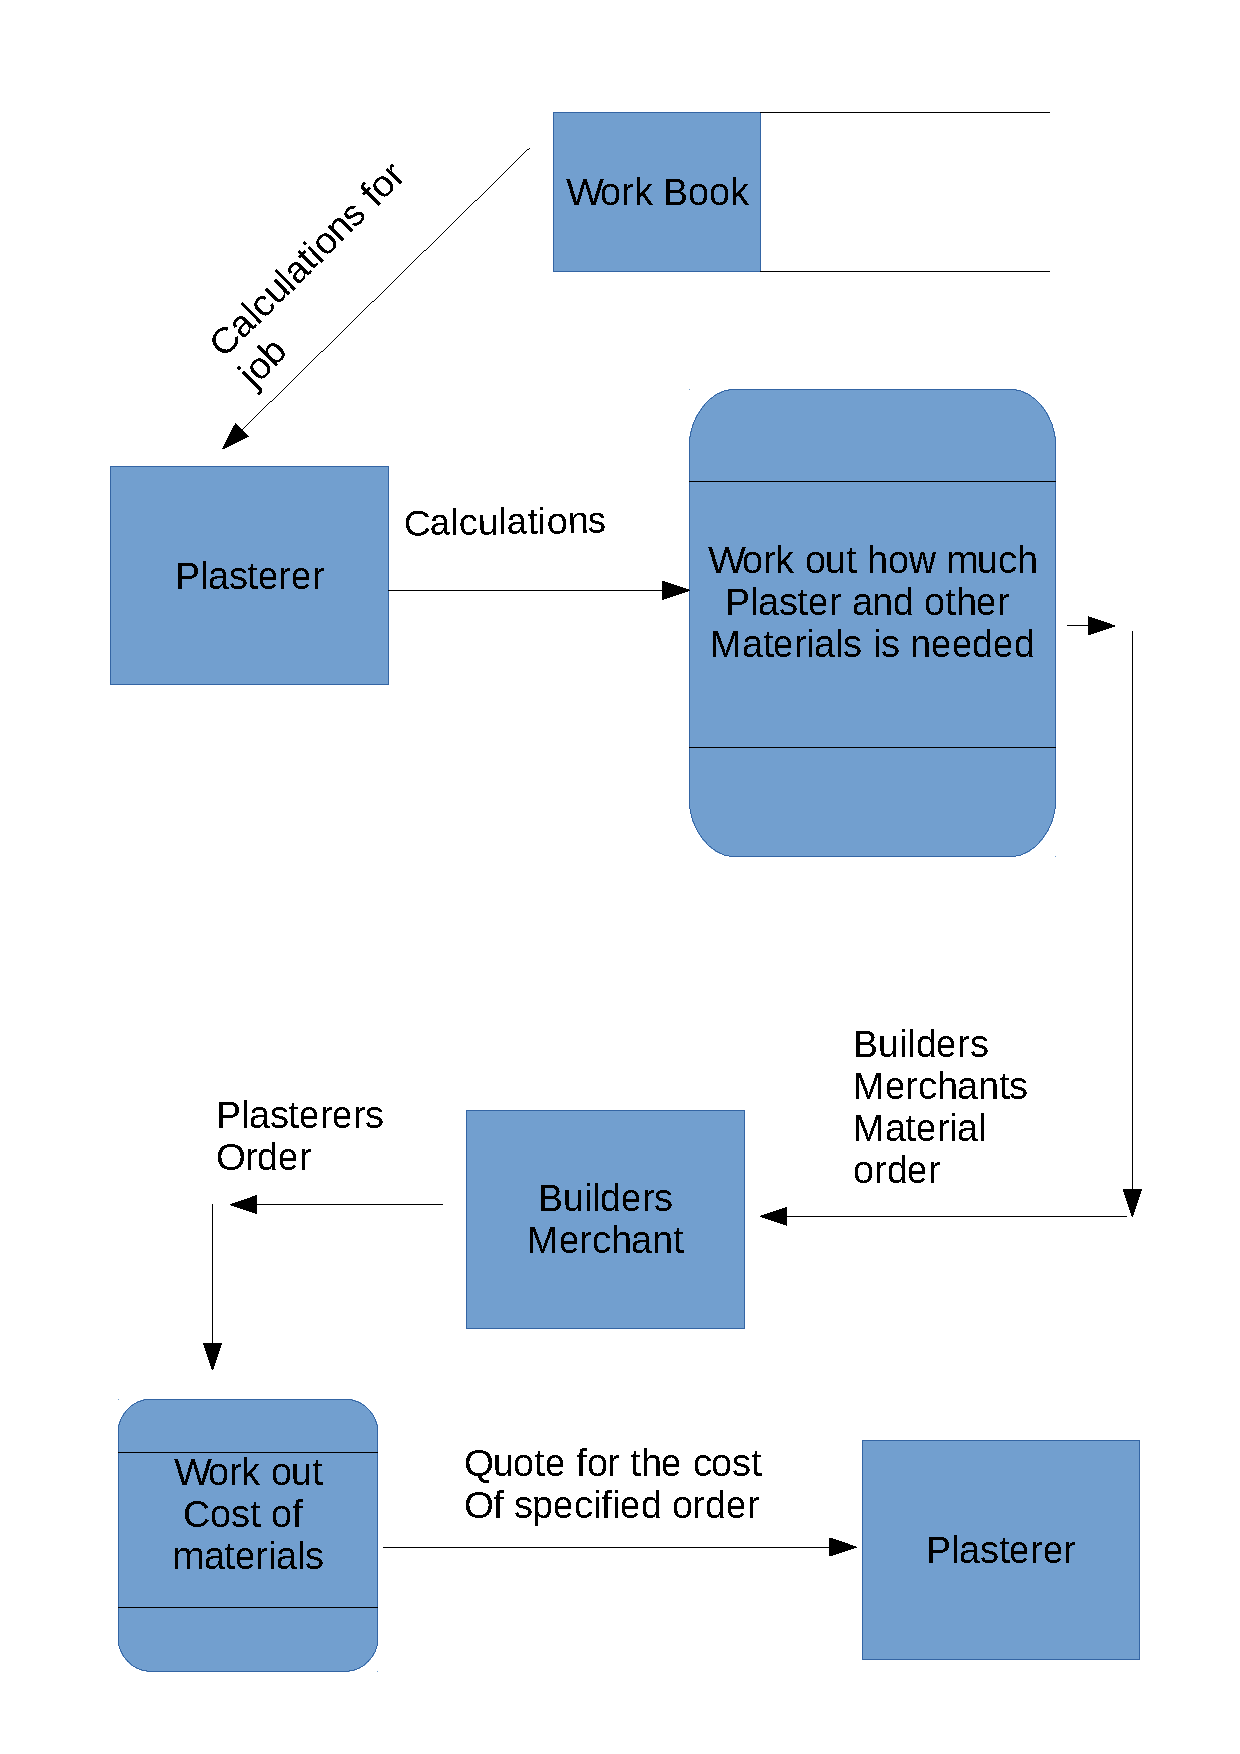
\includegraphics[width=\textwidth]{./Analysis/images/GettingQuoteFromBuildersMerchant.pdf}
    \caption{This shows the data flow when getting a quote for the materials.} \label{fig:getting_materials_data_flow_diagram}
\end{figure}



\begin{figure}[H]
    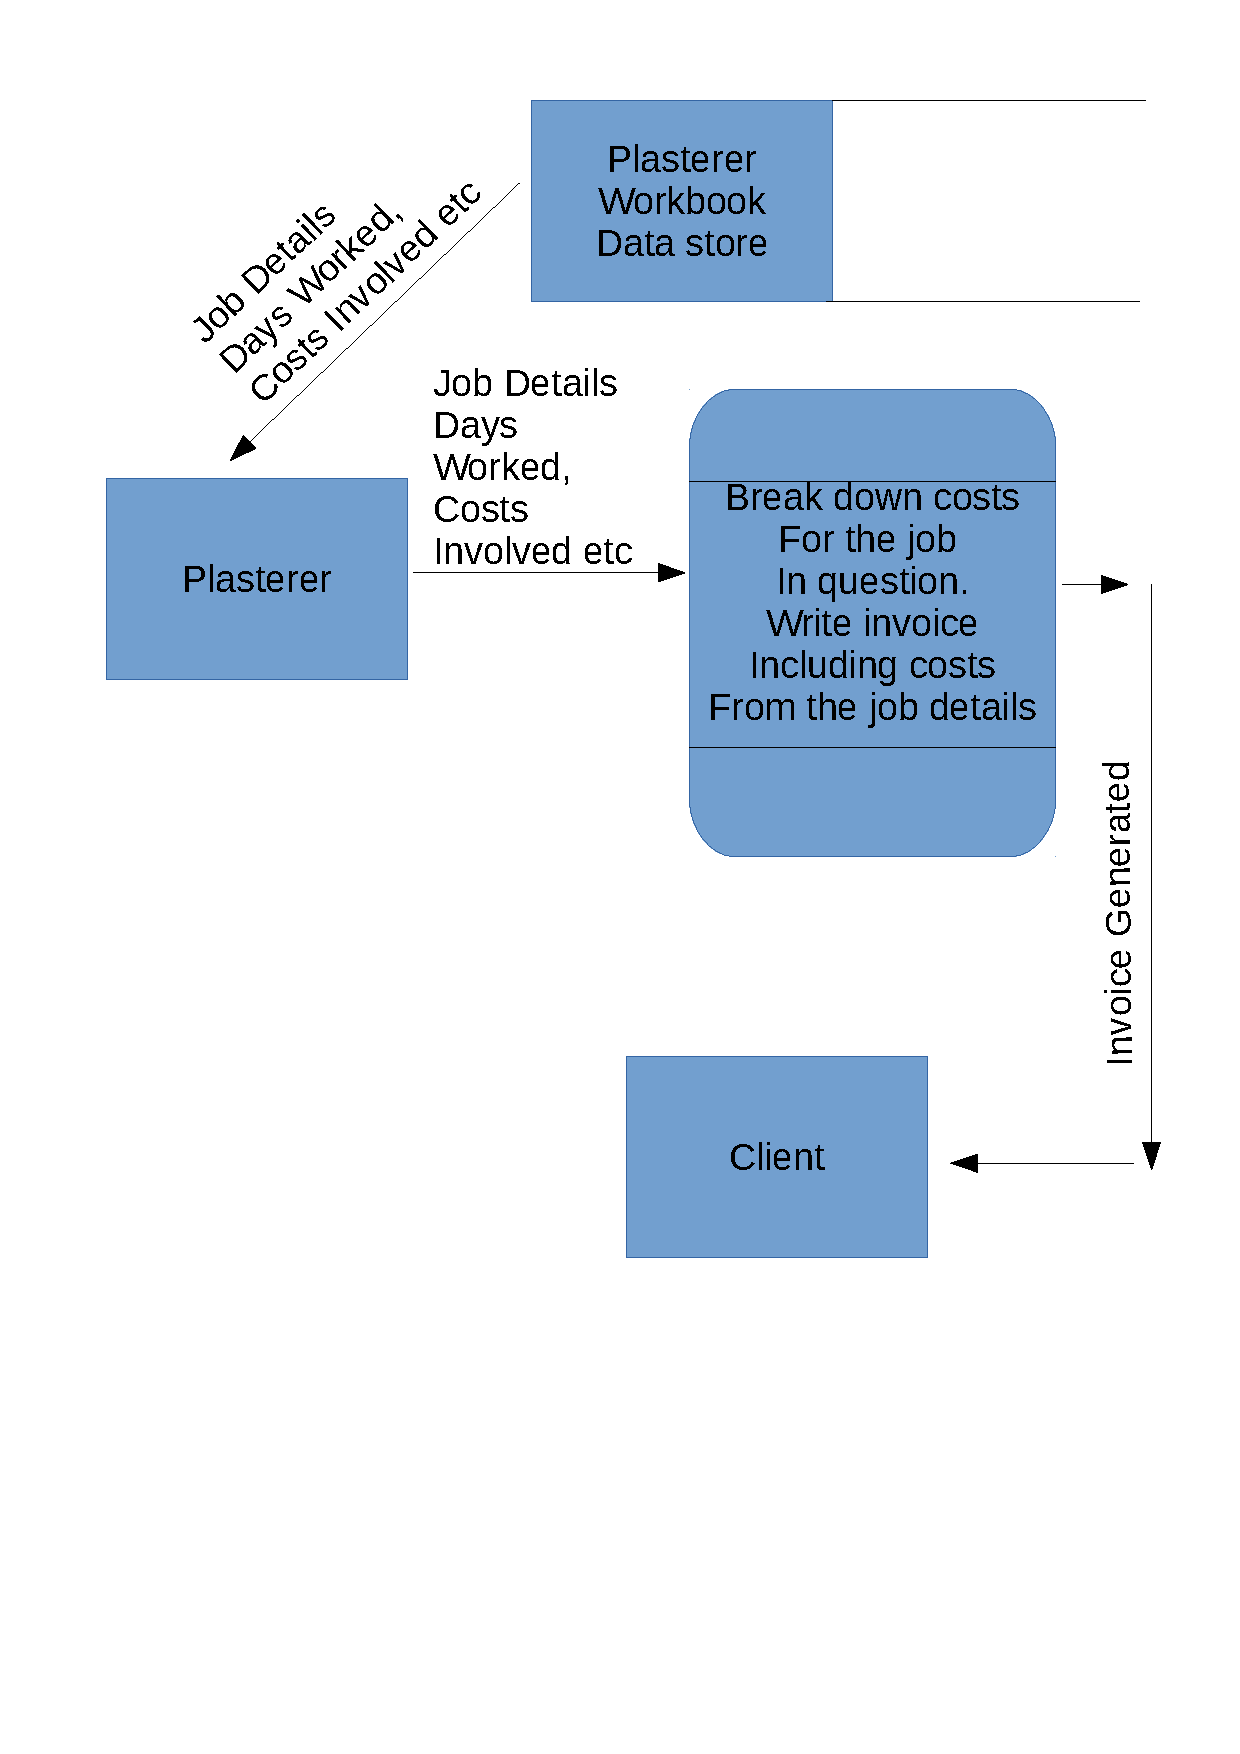
\includegraphics[width=\textwidth]{./Analysis/images/GivingAnInvoiceToClient.pdf}
    \caption{The Data flow when an invoice is given to the client.} \label{fig:invoice_data_flow_diagram}
\end{figure}





\subsubsection{Input Forms, Output Forms, Report Formats}

\pagebreak

%scale the diagrams ?
\begin{figure}[H]
    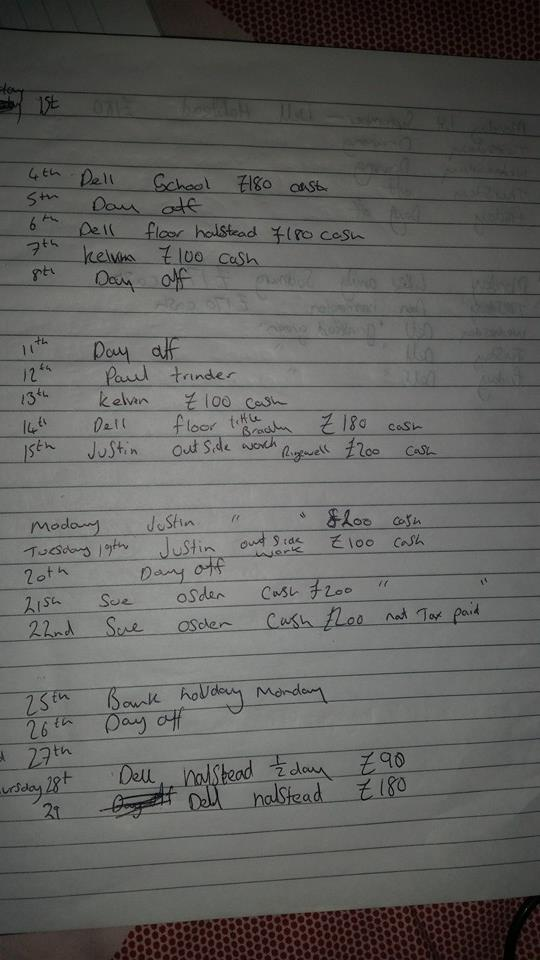
\includegraphics[width=\textwidth]{./Analysis/images/workbookPage.jpg}
    \caption{This is an example of an input form where data is put into the system and is a page from a work book used to store details about jobs.} \label{fig:work_book_page}
\end{figure}

\begin{figure}[H]
    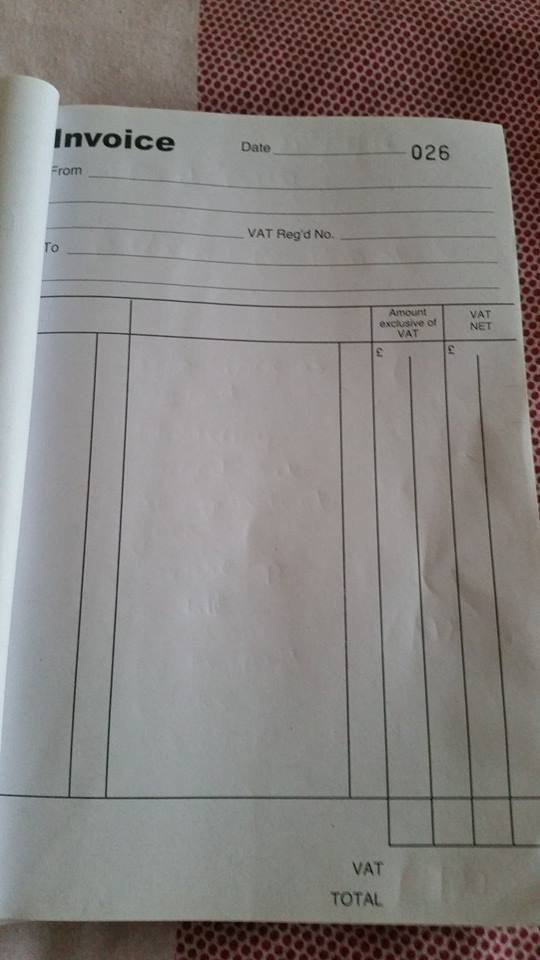
\includegraphics[width=\textwidth]{./Analysis/images/invoice.jpg}
    \caption{This is an example of an invoice output form which is given to clients.} \label{fig:invoice}
\end{figure}

\begin{figure}[H]
    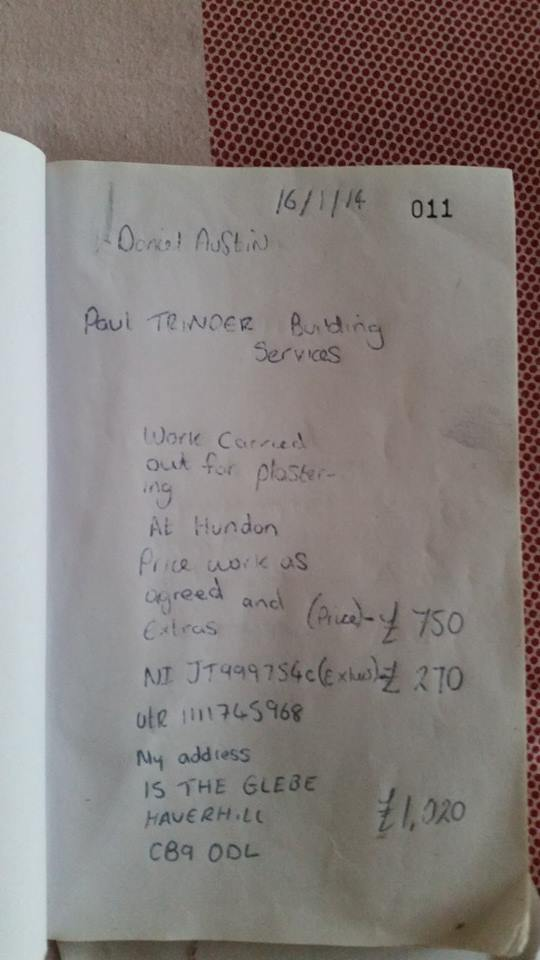
\includegraphics[width=\textwidth]{./Analysis/images/invoice2.jpg}
    \caption{Here is an illustration of the type of information which goes on an invoice to the client.} \label{fig:invoice}
\end{figure}


\begin{figure}[H]
    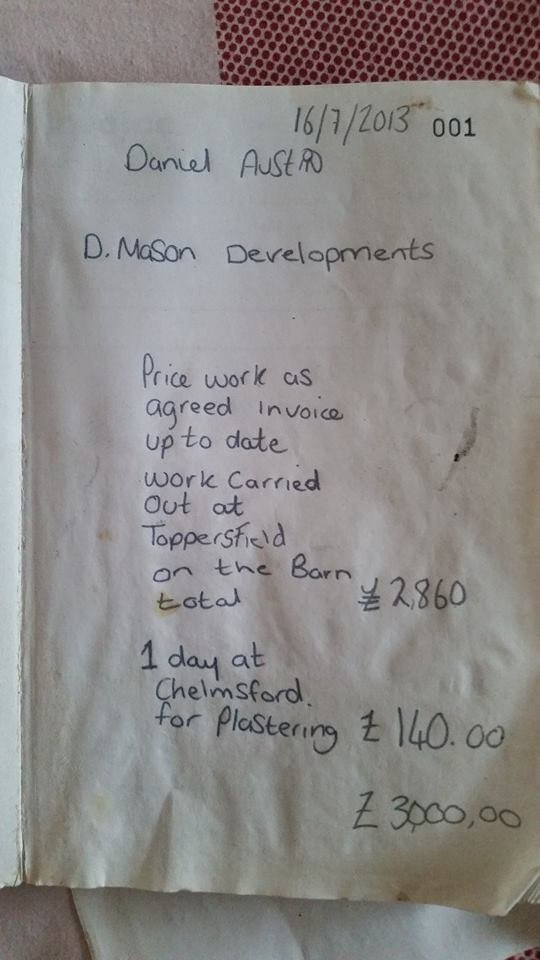
\includegraphics[width=\textwidth]{./Analysis/images/invoice3.jpg}
    \caption{This is also another example of an invoice which is given to a client.} \label{fig:invoice}
\end{figure}

\subsection{The proposed system}

\subsubsection{Data sources and destinations}



\begin{flushleft}
\begin{longtable}{|p{3cm}|p{3cm}|p{3cm}|p{3cm}|}
\hline
\textbf{Source} & \textbf{Data} & \textbf{Data Type} & \textbf{Destination}  \\ \hline
Client & Firstname & String/text & Plasterer \\ \hline 
Client & Surname   & String/text & Plasterer \\ \hline
Client & AddrLine1 & String/text & Plasterer \\ \hline
Client & AddrLine2 & String/text & Plasterer \\ \hline
Client & AddrLine3 & String/text & Plasterer \\ \hline
Client & AddrLine4 & String/text & Plasterer \\ \hline
Client & PostCode  & String/text & Plasterer \\ \hline
Client & Email     & String/text & Plasterer \\ \hline
Client & MobNumber & String/text & Plasterer \\ \hline   
Plasterer & ClientID & Integer & Client Records \\ \hline
Plasterer & Firstname & String/text & Client Records \\ \hline 
Plasterer & Surname   & String/text & Client Records \\ \hline
Plasterer & AddrLine1 & String/text & Client Records \\ \hline
Plasterer & AddrLine2 & String/text & Client Records \\ \hline
Plasterer & AddrLine3 & String/text & Client Records \\ \hline
Plasterer & AddrLine4 & String/text & Client Records \\ \hline
Plasterer & PostCode  & String/text & Client Records \\ \hline
Plasterer & Email     & String/text & Client Records \\ \hline
Plasterer & MobNumber & String/text & Client Records \\ \hline   
Job site & JobID & Integer & Job Records \\ \hline
Job site & ClientID & Integer & Job Records \\ \hline
Job site & Job Desc & Text & Job Records \\ \hline
Job site & AddrLine1 & String/text & Job Records \\ \hline
Job site & AddrLine2 & String/text & Job Records \\ \hline
Job site & AddrLine3 & String/text & Job Records \\ \hline
Job site & AddrLine4 & String/text & Job Records \\ \hline
Job site & PostCode  & String/text & Job Records \\ \hline
Job site & Job Total Price & Currency & Job Records \\ \hline
Job site & JobPaid     & Boolean & Job Records \\ \hline
Job site & JobDaysWorked & Integer & Job Records \\ \hline
Job site & JobComplete & Boolean & Job Records \\ \hline   
Plasterer & AppointmentID & Integer & Appointment Records \\ \hline
Plasterer & ClientID & String/text & Appointment Records \\ \hline 
Plasterer & PlastererID & String/text & Appointment Records \\ \hline
Plasterer & AppointmentDate & String/text & Appointment Records \\ \hline
Plasterer & AppointmentTime & String/text & Appointment Records \\ \hline
Plasterer & AppointmentAddr1 & String/text & Appointment Records \\ \hline
Plasterer & AppointmentAddr2 & String/text & Appointment Records \\ \hline
Plasterer & AppointmentAddr3 & String/text & Appointment Records \\ \hline
Plasterer & AppointmentAddr4 & String/text & Appointment Records \\ \hline







\end{longtable}





\end{flushleft}



\subsubsection{Data flow diagrams}

\begin{figure}[H]
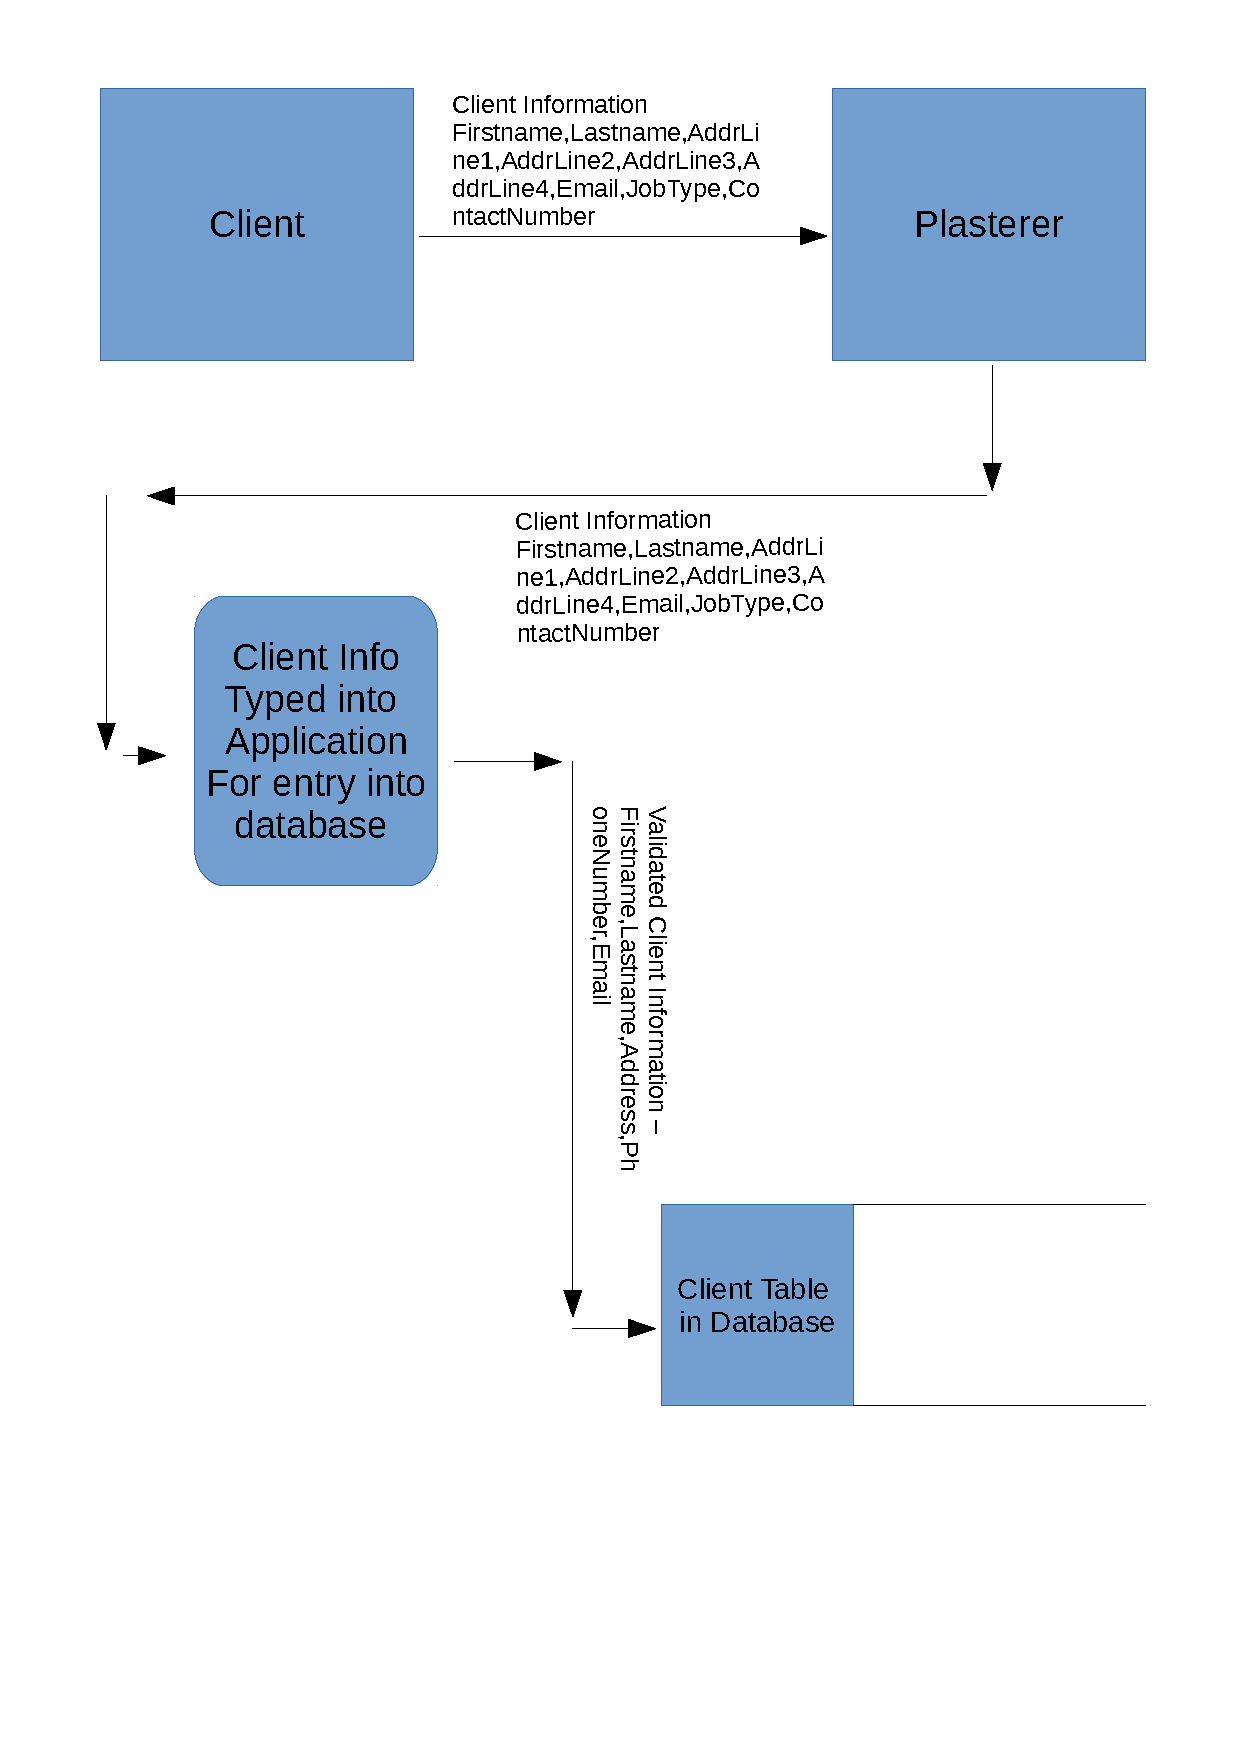
\includegraphics[width=\textwidth]{./Analysis/images/proposedSystemGainingClientInfo.pdf}
    \caption{This data flow diagram signifies the flow of data in the proposed system when gaining a new clients info.} \label{fig:proposed_system_dfd_1}
\end{figure}


\begin{figure}[H]
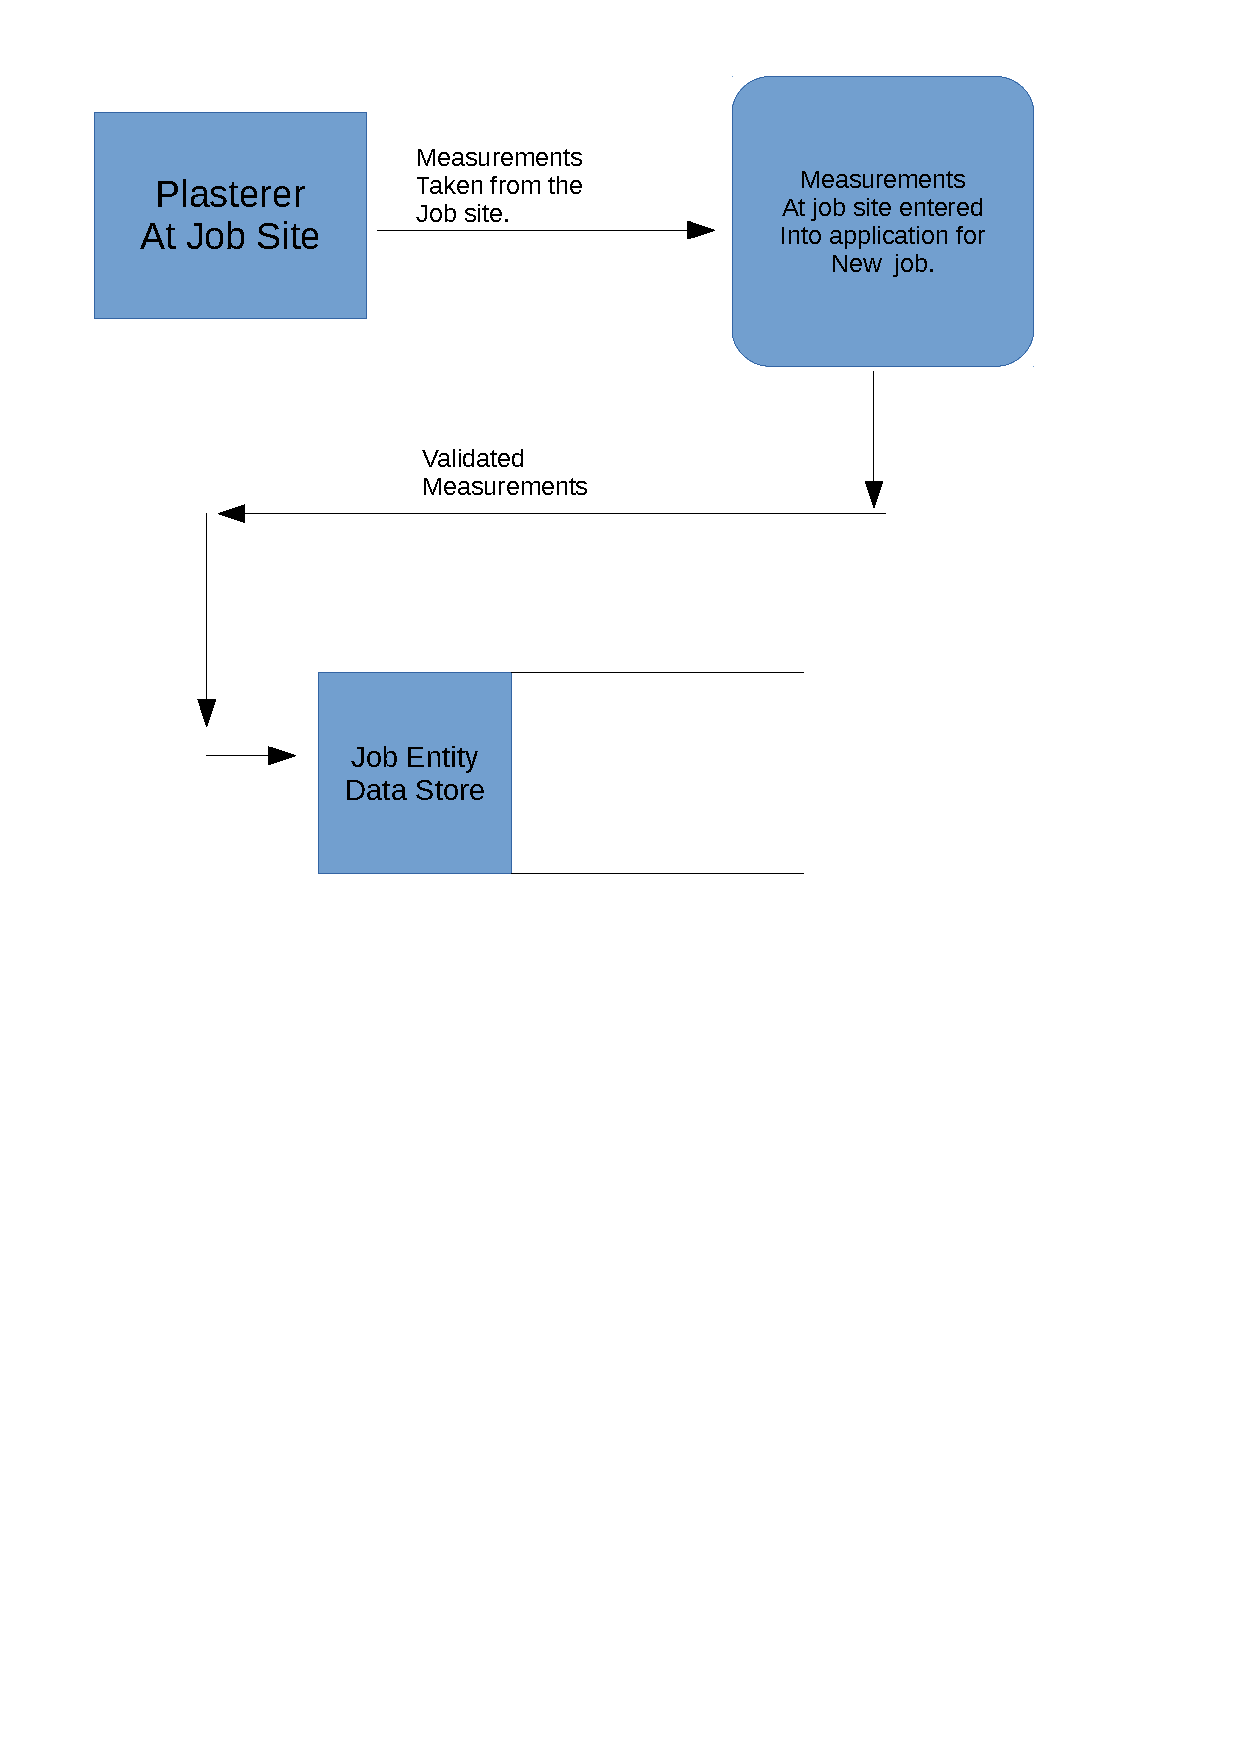
\includegraphics[width=\textwidth]{./Analysis/images/proposedSystemGettingMeasurements.pdf}
    \caption{This data flow diagram signifies the flow of data in the proposed system when collecting the measurements from the job site.} \label{fig:proposed_system_dfd_2}
\end{figure}


\begin{figure}[H]
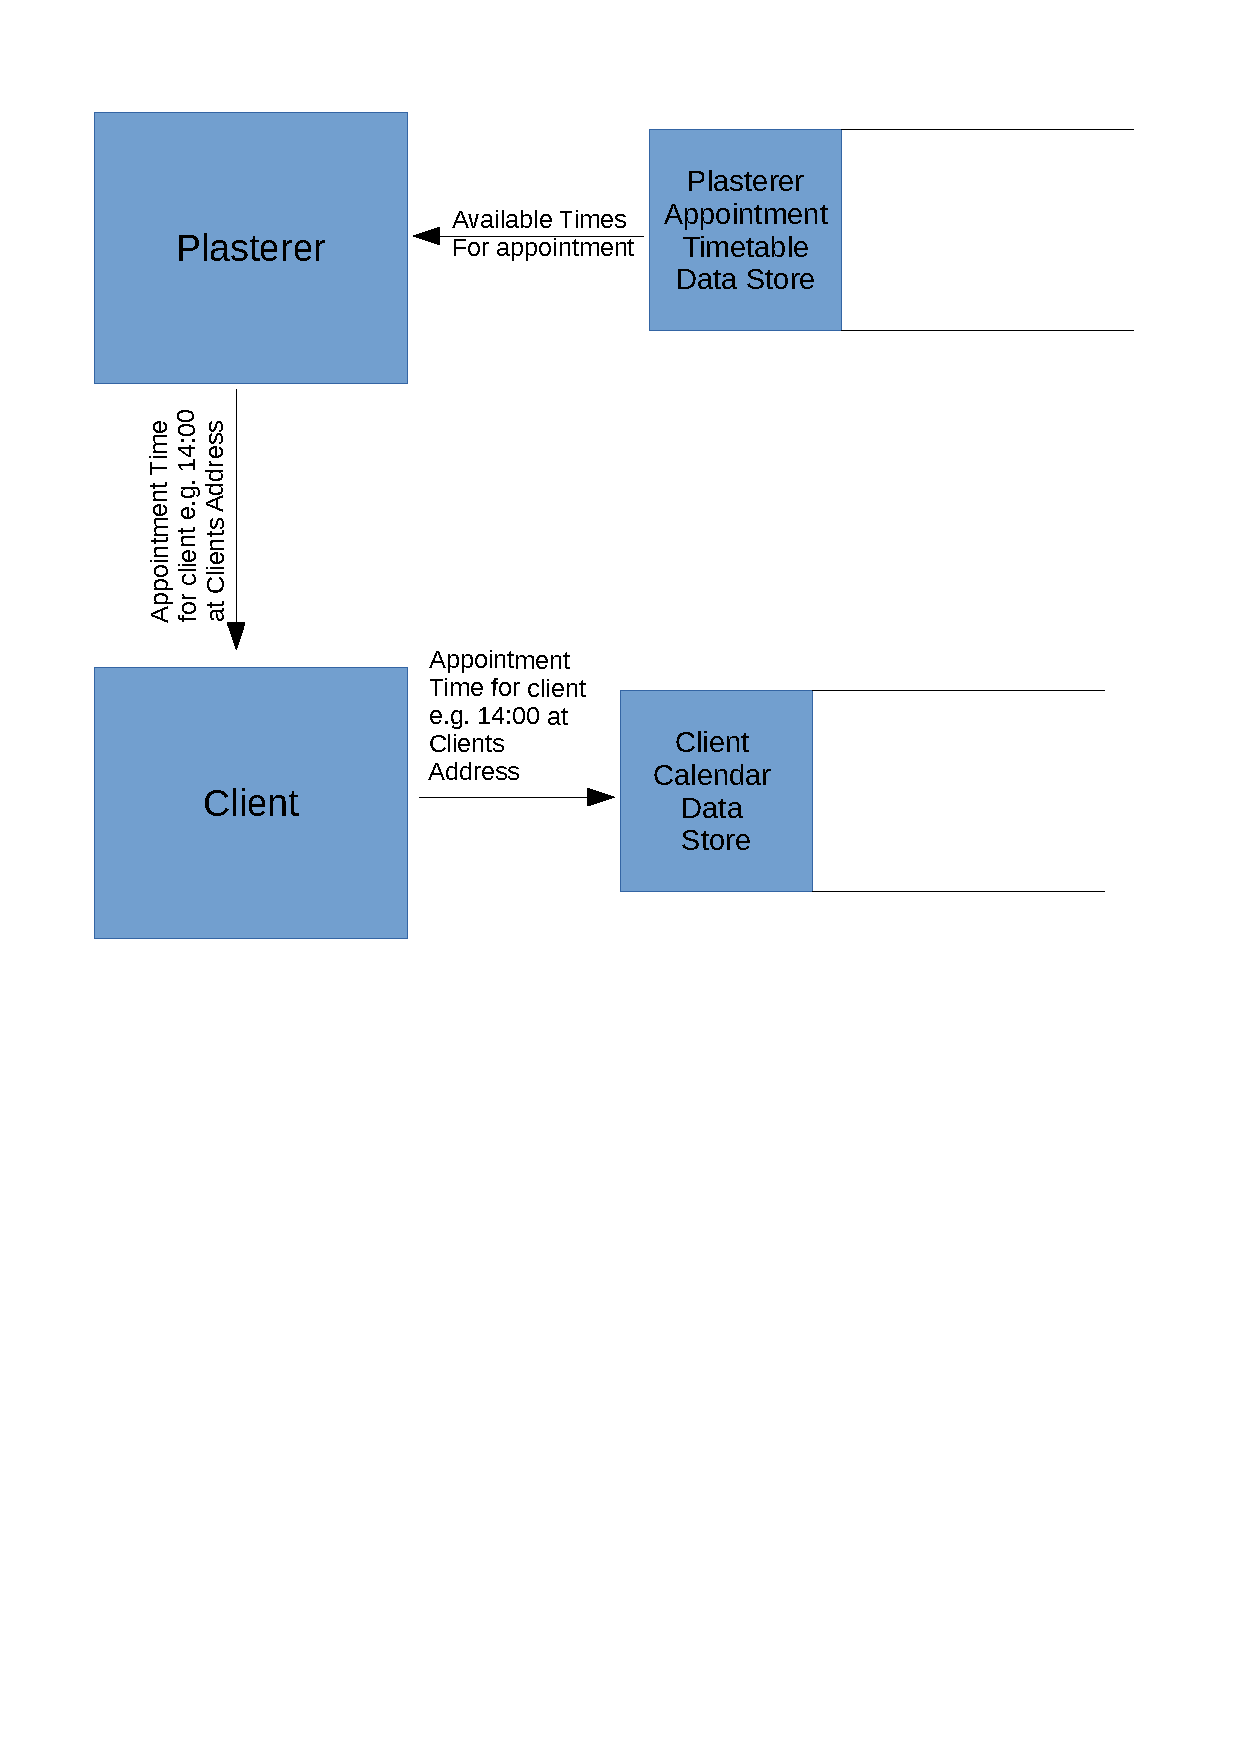
\includegraphics[width=\textwidth]{./Analysis/images/proposedSystemGivingClientAppointmentTime.pdf}
    \caption{This diagram shows the flow of the data in the proposed system when a client is given an appointment time.} \label{fig:proposed_system_dfd_3}
\end{figure}


\begin{figure}[H]
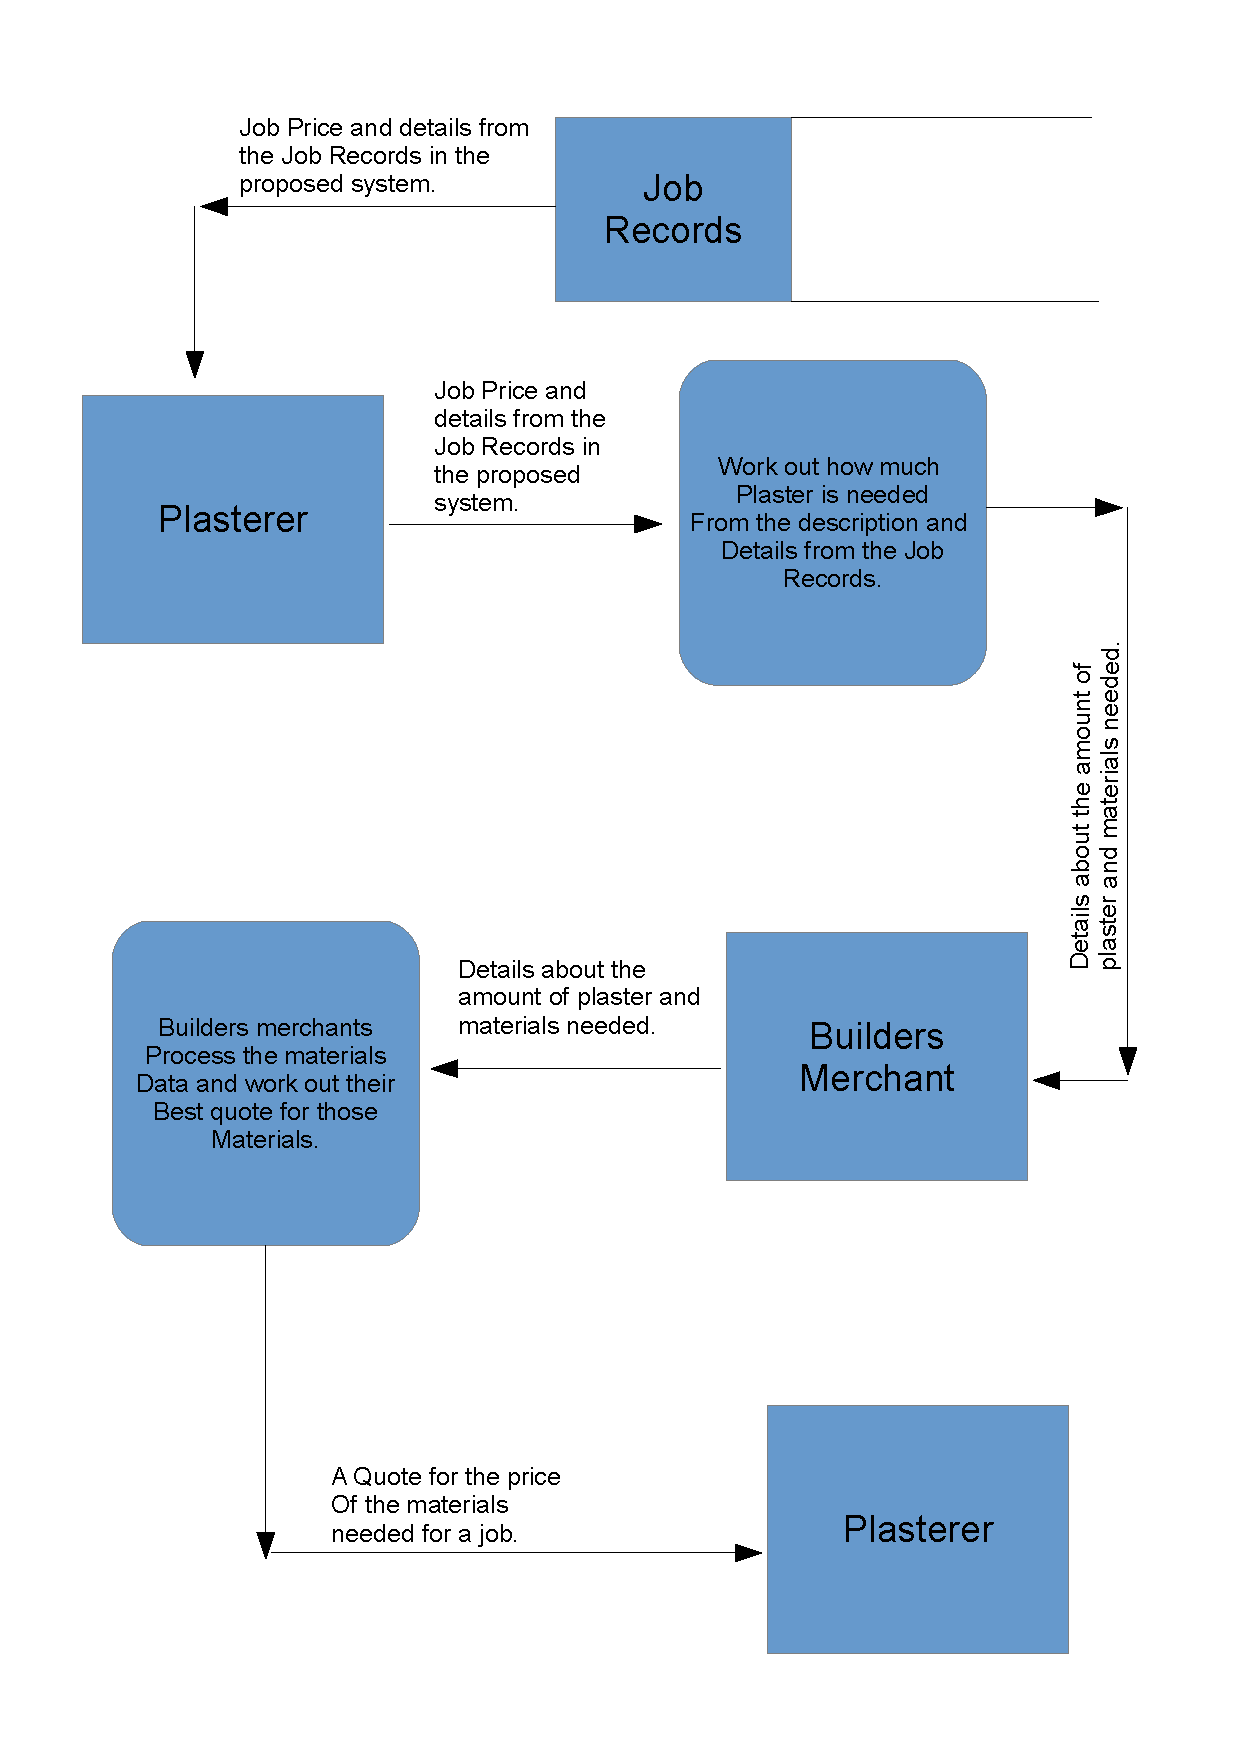
\includegraphics[width=\textwidth]{./Analysis/images/proposedSystemGettingQuoteFromBuildersMerchant.pdf}
    \caption{This diagram shows the flow of the data in the proposed system when the plasterer gets a quote for the materials from the builders merchants.} \label{fig:proposed_system_dfd_4}
\end{figure}

\begin{figure}[H]
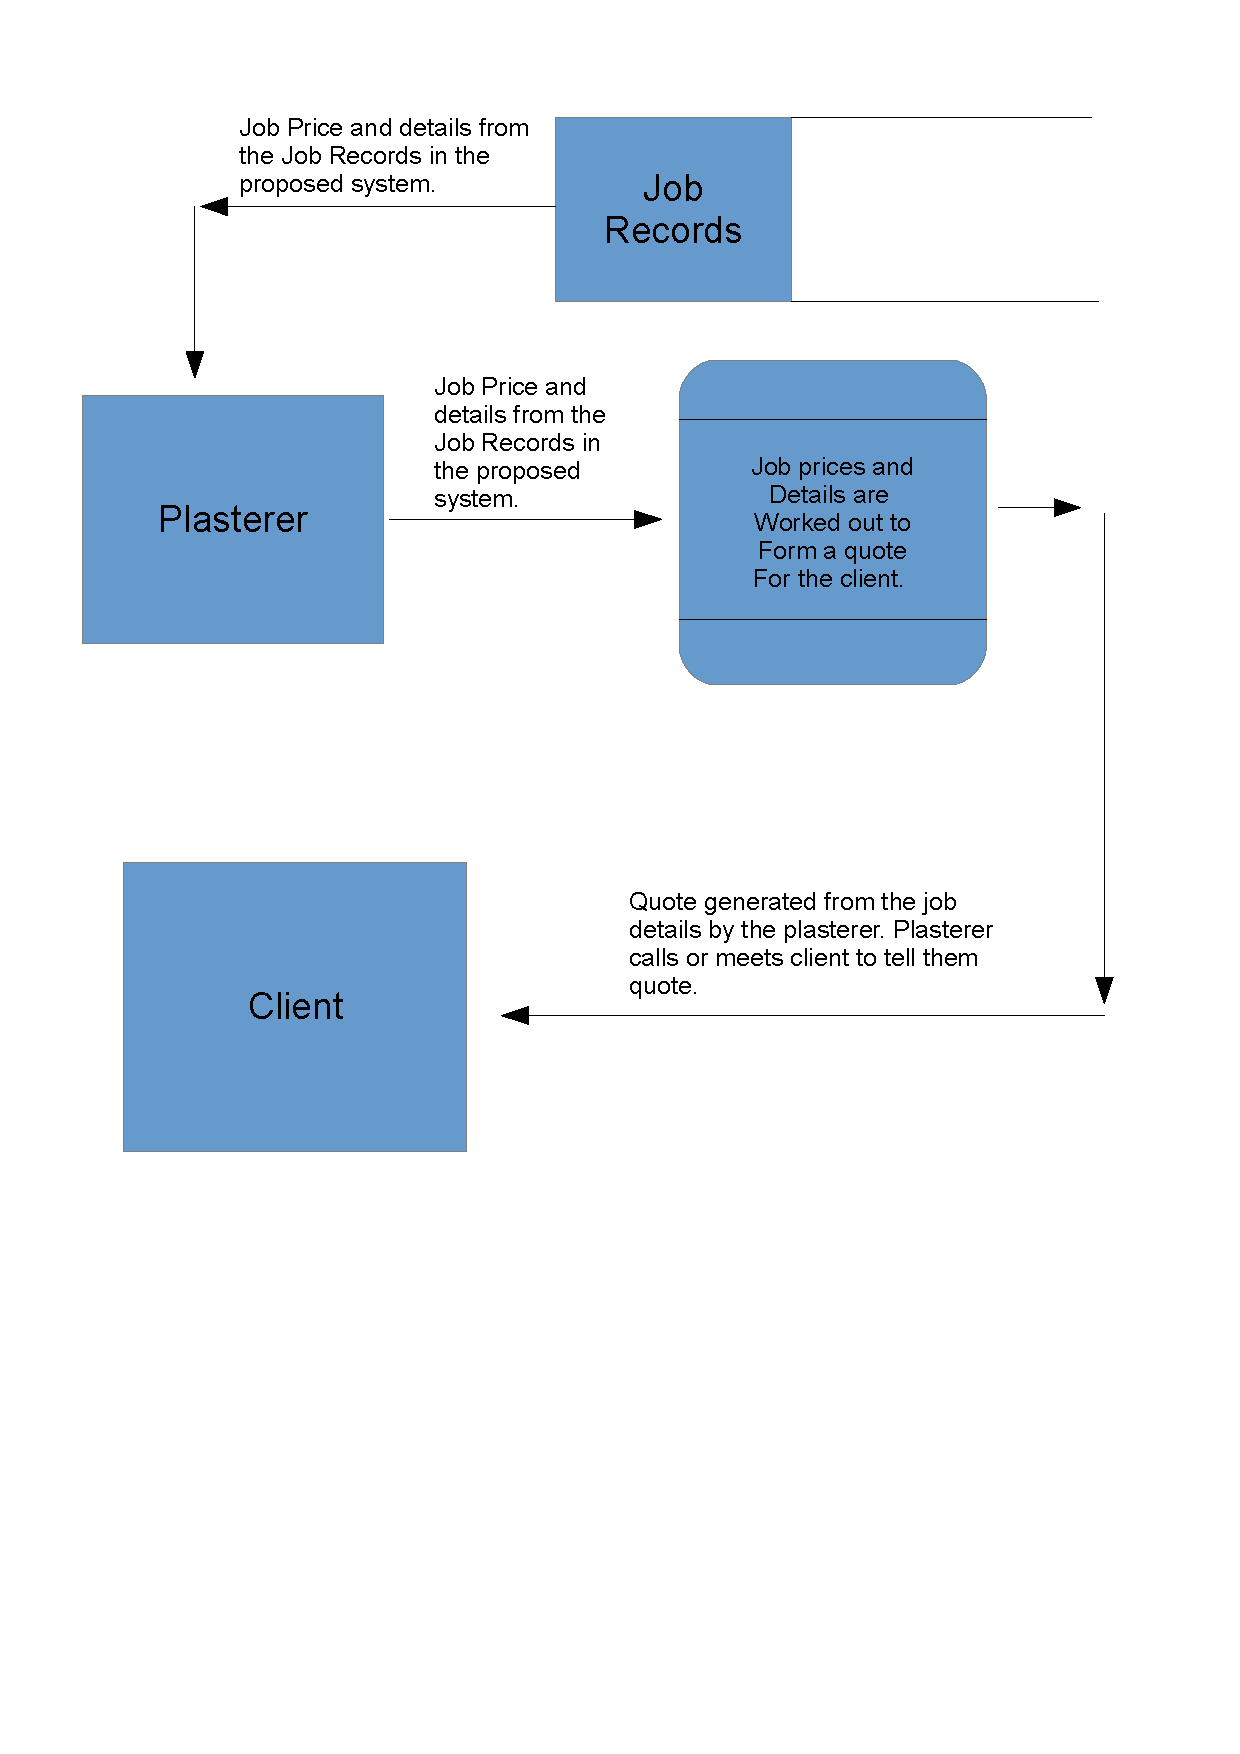
\includegraphics[width=\textwidth]{./Analysis/images/proposedSystemGeneratingQuoteForClient.pdf}
    \caption{This diagram shows the flow of the data in the proposed system when a quote is generated for the client and given to them.} \label{fig:proposed_system_dfd_5}
\end{figure}




\subsubsection{Data dictionary}





\subsubsection{Volumetrics}

\begin{flushleft}

	In the current system Dan only has a few regular clients but it is possible to receive up to 4-5 additional clients each week (mentioned in interviequestion 8). Therefore using the guidline of around 4 clients a week and a trial period for the application of 3 months, there could be upto 48 new clients (4 clients a week x 4 weeks in month x 3 months = 48) added into the database. It would also be useful to add the existing clients from paper so another 50 clients could be added from what is already stored manually. So around 100 clients may be added to the new system. This size can be increased later if necessary. \par

In the job details table each client may have up to 10 or more jobs. Some clients will only have one and some will be recurring customers so will have a few more. In the calculations for minimum storage space I will say that each field takes up 1KB of hard disk space and all together there will be around 50 related fields for each client so:

\begin{itemize}
    \item 100 x 50KB = 5000 KB
	 \item 5000 KB / 1024 = 4.8MB
\end{itemize}
s
If the application took up around 5MB itself then the total space required for the proposed system would be around 9.8MB (4.8MB + 5MB = 9.8MB). Dans computer has plenty of hard disk space that could be used when installing the application. This proposed system would therefore have enough storage space for 100 clients to be added to the client database.


\end{flushleft}



\section{Objectives}

\subsection{General Objectives}

	\begin{itemize}
		\item Clean and easy to use GUI.
		\item Use a database for storing data.
		\item Make it as easy as possible to find data.
		\item Add clients to database.
		\item Make it easy to calculate costs involved.
		\item Sort client data and add search functionality.
		\item Ability to add multiple jobs per client.
	\end{itemize}

\subsection{Specific Objectives}
	
	\textbf{Client Data Store Objectives}
	\begin{itemize}
		\item Ability for Dan to add a client to a database.
		\item Ability for Dan to be able to delete a client from the database if needed.
		\item Dan should be able to modify and append exisitng clients details with and easy to use system.
		\item A search feature that will let Dan filter the database of clients to dfind vital information.

	\end{itemize}
	
	\textbf{Jobs Objectives}
	\begin{itemize}
		\item Dan will be able to add a job which will relate to a client stored in the client entity.
		\item Multiple jobs can be added.
		\item The jobs will contain the job details (description) and address etc (see entity descriptions for more details).
		\item Each job will be able to generate invoices from the data.
		\item The invoice will be able to be sent to the client digitally(by email) or manually (print invoice).
		\item The user will have the ability to edit the details if needed for each job.
	
	\end{itemize}
	
	\textbf{Management features objectives.}
	
		\begin{itemize}
			\item Dan will be able to generate reports between x and y time periods in order to see the amount earned within that period.
			\item A feature will be implemented whereby the user can deduct tax and other specified costs from the amount earned within that period.
			\item Ability to print this pay report and generate a digital versatile copy of the report.
		\end{itemize}	


\subsection{Core Objectives}
	
	\begin{itemize}
		\item The application must store the client details in a database.
		\item The application must be able to add jobs for each client.
		\item The application must be able  modify client and job details.
		\item The application must be able to send an invoice to the client via email.
		\item The application must be able to generate a report for the amount earned within a time period.
	\end{itemize}


\subsection{Other Objectives}

	\begin{itemize}
		\item The application may be able to print an invoice for the client.
		\item The application may be able to send quotes for jobs via email.
		\item The application may be able to print a report for the amount earned within a time period.
	
	\end{itemize}



\section{ER Diagrams and Descriptions}

\subsection{ER Diagram}

\begin{figure}[H]
    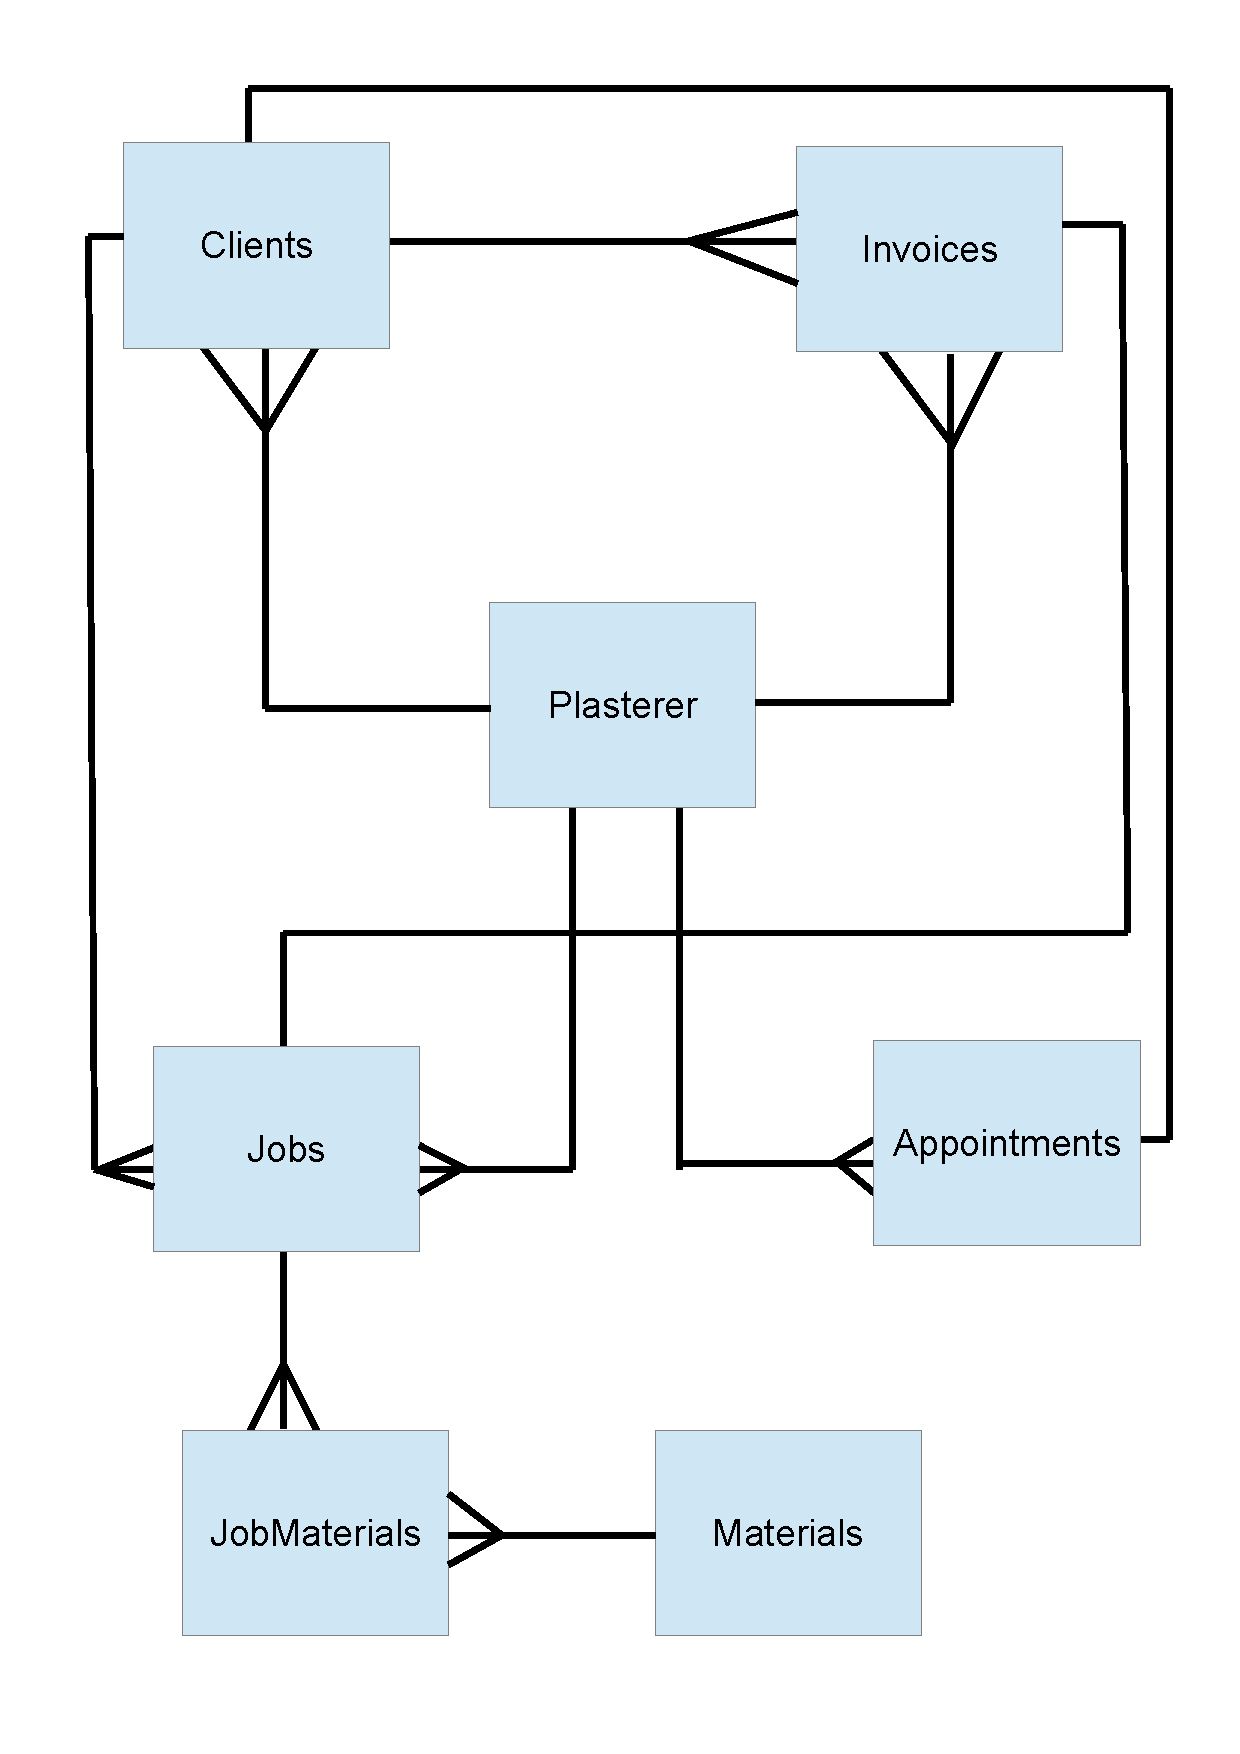
\includegraphics[width=\textwidth]{./Analysis/images/ER-Diagram.pdf}
    \caption{This is the entity relationship diagram for the sqlite3 database.} \label{fig:Entity_Relationship_Diagram}
\end{figure}


\subsection{Entity Descriptions}

\begin{flushleft}

Below are the entity descriptions for the various entites in the proposed system. An \underline{underlined} attribute denotes a primary key and a \emph{emphasised}	attribute signifies a foreign key in the entity.

\end{flushleft}




\begin{center}
	\textbf{Client}(\underline{ClientID}, ClientTitle, ClientFirstName, ClientSurname, ClientAddrLine1, ClientAddrLine2, ClientAddrLine3, ClientAddrLine4, ClientEmail, ClientPhoneNumber, \emph{PlastererID})
\end{center}



\begin{center}
	\textbf{Plasterer}(\underline{PlastererID}, PlastererFirstName, PlastererSurname, PlastererAddrLine1, PlastererAddrLine2, PlastererAddrLine3, PlastererAddrLine4, PlastererEmail,PlastererPhoneNumber, PlastererDailyRate)
\end{center}



\begin{center}
\textbf{Job}(\underline{JobID}, \emph{ClientID}, \emph{PlastererID}, JobDescription, JobAddrLine1, JobAddrLine2, JobAddrLine3, JobDaysWorked JobAddrLine4, JobComplete, JobPaid, \emph{InvoiceID})
\end{center}


\begin{center}
\textbf{Material}(\underline{MaterialID},MaterialName,MaterialPrice)
\end{center}


\begin{center}
\textbf{JobMaterials}(\underline{JobMaterialsID}, \emph{JobID}, \emph{MaterialsID}, JobMaterialsQuantity)
\end{center}


\begin{center}
\textbf{Invoice}(\underline{InvoiceID}, \emph{ClientID}, \emph{JobID}, \emph{PlastererID} InvoiceAmountPreTax, InvoiceAmountAfterTax, InvoiceReceived, InvoiceDate, InvoiceText)
\end{center}



\begin{center}
\textbf{Appointment}(\underline{AppointmentID}, \emph{ClientID}, \emph{PlastererID}, AppointmentDate, AppointmentTime, AppointmentAddrLine1, AppointmentAddrLine2, AppointmentAddrLine3, AppointmentAddrLine4)
\end{center}



\section{Object Analysis}

\subsection{Object Listing}

\textbf{Objects}
	\begin{itemize}
		\item Client
		\item Jobs
		\item Materials
		\item JobsMaterials
		\item Invoices
		\item Appointment
		\item Plasterer
	\end{itemize}

\subsection{Relationship diagrams}



\subsection{Class definitions}





\section{Other Abstractions and Graphs}

\section{Constraints}

\subsection{Hardware}

\begin{flushleft}
	Dan currently has a Toshiba Laptop with the following hardware components:
	
	\begin{itemize}
		\item 6GB DDR3 RAM
		\item Intel 2.0ghz Dual Core Processor
		\item High Resolution 1920 x 1080 Display
		\item 1 TB HDD
		\item Intel Onboard Integrated Graphics
	\end{itemize}

	The specification of Dan's laptop is more than powerful enough and has enough RAM to run the proposed python application alongside multiple other programs that he regularly uses (such as a Web Browser and Media Player). The hard drive has enough storage space to install the application (which will only be around 10MB) so storage is not a problem. The only possible complication when it comes to hardware may be the screen resolution as the application will have to keep within the resolution and be optimized for this screen size and many more to keep the software versatile.
\end{flushleft}

\subsection{Software}

\begin{flushleft}
	Dan is running the Windows 8 operating system on his laptop. The proposed system will need to be able to run on this operating system which is not a problem as the proposed system can easily be packaged into a installation executable which he will be able to run and install the proposed system. This will remove the constraint of not having python natively installed on the system.

\end{flushleft}

\subsection{Time}

\begin{flushleft}
 	Dan is very flexible when it comes to time as he is a freelancer and is in no rush for a replacement to his old system. He does not mind how long the new system takes to be implemented just that it works and functions as expected. Therefore the only time constraint for the proposed system would be the coursework deadline which is Friday 27th March 2015.
\end{flushleft}

\subsection{User Knowledge}

\begin{flushleft}
	Dan has no formal qualifications in IT and has never performed complex computerised tasks. Browsing the internet, watching films and playing music is the extent to which Dan currently uses his laptop. Therefore user knowledge is a possible constraint and the proposed system will need to be easy to navigate and use. This may be achieved by providing a simple non-complex GUI and detailed tutorials/documentation.
\end{flushleft}

\subsection{Access restrictions}

\begin{flushleft}

	The proposed system will not need additional security measures as no one else will be using the system and Dan is the only person that will use the application so different user accounts will not be needed. 

\end{flushleft}

\section{Limitations}

\subsection{Areas which will not be included in computerisation}

	\begin{itemize}
		\item The collection of the measurements from the job site will still have to be done manually so will not be included in computerisation.
		\item Getting the quote for the price of the materials will still be done manually as it will be difficult to computerise as you have to visit the Builders Merchants in person.
	\end{itemize}

\subsection{Areas considered for future computerisation}
	\begin{itemize}
		\item The collection of the measurements, which is currently being done manually, may be implemented using a device which has kinect like sensors, you could scan a room and pick up the measurements of it using just a phone for example. This might be possible.
	\end{itemize}

\pagebreak
\section{Solutions}

\subsection{Alternative solutions}

\pagebreak
\begin{flushleft}
\begin{longtable}{|p{3cm}|p{4cm}|p{4cm}|}
\hline
\textbf{Solution} & \textbf{Advantages} & \textbf{Disadvantages} \\ \hline

Web Application &

{Can be accessed on multiple devices where theres is an internet connection.
Only a web browser required (already installed in most cases).
Can be easier to make it look "pretty" as there are many graphical libraries for the web.
Can use different server side languages to program the backend of the website. (Python (Django),Ruby(RoR)
\linebreak
,PHP(Zend,Magneto)).}&

{Need an internet connection to visit site if not hosted locally.
A web host may need to be purchased.
Need to optimize for different browsers (Internet Explorer, Chrome, Firefox, Safari).
Problems may happen with host which means the client may not be able to access their application (site may be subject to DDOS (may need to purchase Cloudflare or similiar service))}.

\\ \hline

Mobile Phone Application &

Can mean the application is extremely mobile so the client will be able to take the app wherever he goes which may useful to take to jobs.
Client is familiar with using a mobile phone so may be easier for them to use.&

Will take longer to complete.
It is more complex and can be solved easier with a different method.
Client may lose phone which would then result in loss of application.

\\ \hline

Command-Line Application &

No long waiting time for GUI to load.
System resources are not used up as much. &


Can be more complicated, so it seems to the client.
Interface would be less effective and harder to use for the non-technical client.
Errors may occur and look unfamiliar to client.
If laptop is lost/stolen the the program may be lost too so backups need to be kept online (not so much a problem with a web application).

\\ \hline

Spreadsheet &

Can be faster than a application with a GUI to load.
Data can be exported easily.
Queries are easy to run and execute fast. &

No abstraction from the data.
Client would have to familiarise themselves with the syntax for queries.
You can add a lot more features in PyQt and Python Applications.
No GUI to make it easier for the client to control the functions and run queries. 

\\ \hline

PyQt4 GUI and Python3 Application &

Python is easy to write and can therefore get the project done quicker leaving more time for debugging and testing.
The GUI will make it a lot easier for the client to use the application.
With this form of application it can be packaged for Mac,Windows and Linux Systems.
GUI gives a clear visual representation of the applications features. &

Uses python which needs to be packaged with the program as windows does not have Python natively installed but Mac and Linux do.
Writing a GUI is a lot more work than other solutions. 

\\ \hline

\end{longtable}
\label{tab:Alternative Solutions to the problem}
\end{flushleft}



\subsection{Justification of chosen solution}

\begin{flushleft}
	I have chosen to use Python 3 alongside the Qt Framework (PyQt4) to create a standalone application. This is due to the versatility which Python and PyQt4 offers. Using this method to program a solution to my clients problem I will be able to get it done effeciently due to my existing knowledge of Python and I will be able to generate different executables for different operating systems which may be beneficial to the client as he is looking to buy a Apple System. It will also offer a visual representation through the use of GUI as opposed to hard to use Console application approach; which would not be suitable for the client as he does not have enough technical knowledge with computers to understand and use it easily - therefore going for something with a GUI would be a good choice. A web application may have been good but sometimes Dan takes his laptop where there is no internet connection and hosting the site locally would not be feasible. Also there are hidden costs involved with purhcasing a domain and hosting if a web application solution was chosen. A mobile application may have also been good but would have taken longer to accomplish due to the time it takes to develop complex mobile phone applications. A spreadsheet would also not have been the perfect solution as it requires knowledge of writing queries which, due to Dan's lack of technical computer knowledge, he does not have. Therefore I believe that a Python and PyQt4 application would be the best solution to go for.

\end{flushleft}
